%This file will form the basis of my PhD LaTeX thesis document. I guess there should be only a series of include statements, to include each chapter, and global formatting stuff, like nomenclature shortcut commands. 

\documentclass[11pt,titlepage,twoside,a4paper]{report}

%%%%%%%%%%Packages%%%%%%%%%%
\usepackage{thesis}

%\usepackage{layout}    %For previewing page layout only
\usepackage{fancyhdr}

\usepackage{natbib}
\usepackage{graphicx} 
\usepackage{url}      
\usepackage{amsmath}  
\usepackage{subfigure}
\usepackage{amssymb}
\usepackage{array}
\usepackage{fancybox}
\usepackage{color}
\usepackage[figuresleft]{rotating}
\usepackage{longtable}
\usepackage{nextpage}
\usepackage{graphicx}
\usepackage{amssymb}
\usepackage{pifont}
\usepackage{amsmath}
\usepackage{tikz}
\usepackage {longtable} 
\usepackage{tabularx}
\usepackage{epstopdf}
%\usepackage{setspace}
%%%%%%%%%%%%%%%%%%%%%%%%%%%%

%%%%%%%%%%Commands%%%%%%%%%%
%General
\newcommand{\Rey}{\ensuremath{\mathit{Re}}}       %Reynolds number
\newcommand{\St}{\ensuremath{\mathit{St}}}        %Strouhal number
\newcommand\solidrule[1][1cm]{\rule[0.5ex]{#1}{1pt}}
\newcommand\dashedrule{\mbox{\solidrule[1mm]\hspace{1mm}\solidrule[1mm]\hspace{1mm}\solidrule[1mm]\hspace{1mm}}}


% % % % % % Kj stuff % % % % % % % % % % %
\newcommand{\KJ}[1]{{\textcolor{blue}{{\bf{\it{ **KJ: #1 **}}}}}}
\newcommand{\BT}[1]{{\textcolor{green}{{\bf{\it{ **BT: #1 **}}}}}}
\newcommand{\JL}[1]{{\textcolor{red}{{\bf{\it{ **JL: #1 **}}}}}}



\newcommand{\ustar}{\ensuremath{U^{*}}}
\newcommand{\mstar}{\ensuremath{m^{*}}}
\newcommand{\cstar}{\ensuremath{c^{*}}}
\newcommand{\reynoldsnumber}{\ensuremath{Re}}
\newcommand{\massstiff}{\ensuremath{\Pi_1}}
\newcommand{\massdamp}{\ensuremath{\Pi_2}}
\newcommand{\ratio}{\ensuremath{\frac{d}{l}}}
\newcommand{\cy}{\ensuremath{C_{y}}}
% % % % % % % % % % % % % % % % % % % % % % % % % % % % % % %

\newcommand{\pderiv}[2]{\ensuremath{\frac{\partial#1}{\partial#2}}}
\newcommand{\pderivsq}[2]{\ensuremath{\frac{\partial^2#1}{\partial#2^2}}}
\newcommand{\divergence}[1]{\ensuremath{\nabla\cdot#1}}
\newcommand{\grad}[1]{\ensuremath{\nabla #1}}
\newcommand{\gradsq}[1]{\ensuremath{\nabla^{2}#1}}

\newcommand{\vecu}{\ensuremath{\mathbf{u}}}
\newcommand{\vecV}{\ensuremath{\mathbf{V}}}
\newcommand{\pres}{\ensuremath{p_{f}}}
\newcommand{\Pres}{\ensuremath{P}}

\newcommand{\density}{\ensuremath{\rho}}
\newcommand{\kinvis}{\ensuremath{\nu}}
\newcommand{\dynvis}{\ensuremath{\mu_{v}}}
\newcommand{\Ufree}{\ensuremath{U}}
\newcommand{\diam}{\ensuremath{D}}
\newcommand{\accframe}{\ensuremath{\frac{\mathrm{d}\Vcyl}{\mathrm{d}\tau}}}
\newcommand{\damping}{\ensuremath{\zeta}}
%\newcommand{\ystar}{\ensuremath{y^{*}}}
\newcommand{\kstar}{\ensuremath{k^{*}}}
\newcommand{\Vint}{\ensuremath{\vecV^{*}}}
\newcommand{\Vintint}{\ensuremath{\vecV^{**}}}
\newcommand{\Vn}{\ensuremath{\vecV^{(n)}}}
\newcommand{\Vnext}{\ensuremath{\vecV^{(n+1)}}}
\newcommand{\Vcyl}{\ensuremath{\mathbf{V}_{\mathit{cyl}}}}
\newcommand{\perV}{\ensuremath{\mathbf{v}^{\prime}}}
\newcommand{\period}{\ensuremath{T}}

\newcommand{\mone}{\ensuremath{M1}}
\newcommand{\mtwo}{\ensuremath{M2}}
\newcommand{\mthree}{\ensuremath{M3}}
\newcommand{\mfour}{\ensuremath{M4}}

\newcommand{\upert}{\ensuremath{u^{\prime}}}
\newcommand{\vpert}{\ensuremath{v^{\prime}}}
\newcommand{\wpert}{\ensuremath{w^{\prime}}}
\newcommand{\ppert}{\ensuremath{p^{\prime}}}

\newcommand{\ubase}{\ensuremath{u}}
\newcommand{\vbase}{\ensuremath{v}}

\newcommand{\compone}{\ensuremath{\xi}}
\newcommand{\comptwo}{\ensuremath{\eta}}
\newcommand{\jacobian}{\ensuremath{\mathbf{J}}}

\newcommand{\Vtrial}{\ensuremath{\mathbf{V}_{trial}}}
\newcommand{\Ptrial}{\ensuremath{P_{trial}}}
\newcommand{\residual}{\ensuremath{\mathbf{R}}}
\newcommand{\normal}{\ensuremath{\mathbf{n}}}
\newcommand{\ycyl}{\ensuremath{y_{cyl}}}
\newcommand{\ltwo}{\ensuremath{\mathrm{L}_{2}}}
%%%%New commands arising from driven oscillation chapter%%%%%%%%%%%%%%%%%%%
\newcommand{\clifta}{\ensuremath{C_{L_{a}}}}
\newcommand{\cliftv}{\ensuremath{C_{L_{v}}}}
\newcommand{\phasev}{\ensuremath{\phi_{v}}}
\newcommand{\phasep}{\ensuremath{\phi_{p}}}
\newcommand{\liftf}{\ensuremath{F_{\mathit{lift}}}}
\newcommand{\vcyl}{\ensuremath{\mathbf{v}_{cyl}}}
\newcommand{\clift}{\ensuremath{C_{L}}}

% % % % % % Chap- freq % % % % % % % %
\newcommand{\freq}{\ensuremath{f}}
\newcommand{\freqqss}{$f_{QSS}$}
\newcommand{\freqdns}{$f_{DNS}$}
\newcommand{\freqlin}{$f_{lin}$}

%%%%%%%%%%%%Document formatting: Margins, spacing, etc%%%%%%%%%%%%%%%%%%%%%
\renewcommand{\baselinestretch}{1.5}    %Spacing
\renewcommand{\shadowsize}{3pt}         %Shadowbox shadow depth
\setcounter{tocdepth}{4}                %Table of contents levels

\setlength{\topmargin}{0pt}
\setlength{\textheight}{634pt}
\setlength{\textwidth}{431pt}
\setlength{\marginparwidth}{60pt}
\setlength{\evensidemargin}{0pt}

\pagestyle{fancy}                       %To invoke fancy headers and footers
\fancyfoot{}
\fancyfoot[RO]{\hfill \thepage \hspace{0.05\textwidth}}
\fancyfoot[LE]{\hspace{0.05\textwidth}\thepage \hfill}

\fancyhead{}
\fancyhead[LE]{\leftmark}
\fancyhead[RO]{\rightmark}
\renewcommand{\headrulewidth}{0.4pt}
\renewcommand{\footrulewidth}{0.4pt}

\renewcommand\chaptermark[1]{\markboth{\thechapter. \MakeUppercase{#1}}{}}
\renewcommand\subsectionmark[1]{\markright{\thesubsection. \MakeUppercase{#1}}{}}

\newcommand{\myclearpage}{\thispagestyle{empty}\cleartoevenpage\thispagestyle{empty}\cleartooddpage}
\newcommand{\hilight}[1]{\colorbox{yellow}{#1}}
% % % % % % % % % % % %
%\newenvironment{dedication}
%
%{\vspace{6ex}\begin{quotation}\begin{center}\begin{em}}
%			{\par\end{em}\end{center}\end{quotation}}


%%%%%%%%%%%%The document%%%%%%%%%%%%%%%%%%%%%%%%%%%%%%%%%%%%%%%%%%%%%%%%%%%

\begin{document}
\pagenumbering{roman}
\begin{titlepage}
\noindent\rule{\textwidth}{1.5pt}
\begin{flushright}
\LARGE
{\sc A Numerical Investigation of The Energy Transfer of A Body Under Fluidelastic Galloping} \\

\noindent\rule{\textwidth}{1.5pt}

\LARGE
\vspace{30mm}
{\sc By H.G.K.G Jayatunga}
\vspace{30mm}

\normalsize
{\sc A thesis submitted to Monash University in fulfilment of the requirements for the Degree of}

\vspace{5mm}
\LARGE
{\sc Doctor of Philosophy}

\vspace{15mm}
\normalsize
Department of Mechanical Engineering\\
Monash University\\
October 2015
\end{flushright}

\end{titlepage}

\myclearpage

%%%%%%%%%%%%Dedications here%%%%%%%%%
%\chapter*{Statement of originality}

This thesis contains no material that has been accepted for the award of a degree or diploma in this, or any other, university. To the best of the candidate’s knowledge and belief, this thesis contains no material previously published or written by another person except where due reference is made in the text.

\vspace{20mm}

\begin{flushright}
\solidrule\solidrule\solidrule\solidrule\solidrule\\
Kasun Gayantha Jayatunga\\
October 2016
\end{flushright}
%\myclearpage
%\chapter*{Abstract}


This thesis investigates the potential of energy harvesting through fluid-elastic galloping through studying the energy transfer between the body and the fluid.

This was carried out by numerically integrating a previously derived Quasi-Steady State (QSS), and via Direct Numerical Simulations (DNS) of the fluid-structure system.

A review of the literature identifies a need for new scaling parameters to better represent fluid-elastic galloping. New governing non-dimensional parameters for galloping namely, the combined mass-stiffness, \massstiff\, and the combined mass-damping \massdamp\ are formulated using natural time scales of the linearised QSS model. These new dimensionless groups provide a far better collapse of the predicted power output from the galloping of a square cross section in comparison with the classical parameters, regardless of whether the data comes from the QSS or DNS models. These time scales also provide a linear estimate of the frequency of the system, which is shown to match the frequency measured during the DNS simulations while $\massstiff > 10$.

A comparison between the quasi-steady state and direct numerical simulation data, reveals that the quasi-steady state model provides a good approximation of the power output at high \massstiff. However, the QSS approximation deviates from the DNS predictions at low values of \massstiff\ because the QSS model does not model vortex shedding which becomes more significant as \massstiff\ decreases. However, the QSS model provides a reasonable prediction of the value of \massdamp\ at which maximum power is produced. Both the error in predicted maximum power between the QSS and the DNS models and the relative power of the vortex shedding are quantified and scale approximately to $1/\sqrt{\massstiff}$ .

A semi-empirical search for an optimal body cross section for the extraction of energy is also presented. A hybrid rectangular/triangular body is used, to deliberately test the hypothesis that inhibition of the reattachment of the shear layers can promote large forces, velocities, and therefore energy extraction. It is shown that two features control the energy extraction: the proximity of the shear layer to the body; the velocity of the flow in the shear layers. Both can be controlled by the amount of tapering of the afterbody, and a balance needs to be found between the two to optimize the geometry for energy extraction.

Comparison of results from the QSS and DNS models shows similar trends of maximum power being increased as the body becomes more tapered. However, the difference between the QSS and DNS models increases exponentially as the tapering is increased. Inspection of time averaged flow-field data show that the flow in the true fluid-structure situation is not quasi-static, violating the primary assumption of the QSS model. However, the QSS model still provides a reasonable initial qualitative approximation to design galloping energy harvesting systems. 

%\myclearpage
\chapter*{Acknowledgments}

I would like to express my deepest gratitude to my supervisors, Dr. Tan Boon Thong (Dr. Kenny) and Dr Justin Scott Leontini. Dr. Kenny thank you for entertaining me when I was having difficulties. Dr Justin, for explaining me complicated concepts and helping, guiding and providing words of encouragement when I was going through tough situations. I would like to thank both my supervisors for training me to conduct quality research and teaching me proper research techniques.

My warmest gratitude goes to the administrator of the Monash High-performance computer facility (SUN grid), Philip Chan for helping me out immensely and facilitating to carry out my simulations. Mention must be made to Monash University Malaysia for providing me with the scholarship to pursue my PhD. 
 
I would like to thank my closest friends Nishan and Hasuli who were pseudo-siblings for me from undergraduate level. Thank you for the support and encouragement. I would like to extend my thanks to Rangika and Devangi. Dr Anuja Dharmarathna, thank you for all the support, guidance and treating me as your own son when I needed help.

My Deepest gratitude goes out to my close friends in Monash Malaysia for helping me out, providing support and being there for me when I was going through very tough situations. 

I am indebted for the support provided by my family. Amma, Thatha, Akki, Ayya and Sanula (``Johnny"). Amma thank you for firmly telling me that `` A PhD has to be earned...!". A special thank goes out to Saranga for all the support you provided. My gratitude extends to Mr Nishantha Ranasinghe (Nishantha Ayya) for providing me strength and encouragement.
\\
\\
\\
Last but definitely not least, I am much indebted to Mrs Malin Bamunuarachchi for the blessings, prayers and the encouragement given to me when I hit ``rock-bottom"  and was on the verge of giving up. Thank you madam.    

 

  

  
%\myclearpage
%\begin{titlepage}
\chapter*{Dedication}
	
	\par\vspace*{.23\textheight}{\centering \Large\emph{`` To Mrs. Malin Bamunuarachchi; whom without, this work would have never seen the light of day. Thank you madam; for your prayers, blessings, guidence, kind words of encourgaement and above all, believeing in me and giving me strength to get back up, when I myslef have given up hope...."}\par}
	%\vspace*{\stretch{2.0}}
%\end{titlepage}


\chapter*{A list of publications related to this thesis}


{\sc Jayatunga, H. G. K. G., Tan, B.T \& Leontini, J.S.}  2015
A study on the energy transfer of a square prism under fluid-elastic galloping {\em Journal of Fluids and Structures\/} {\bf 55},384--397.
\vspace{5mm}


\hspace{-\parindent}{\sc Leontini, J.S., Zhao, J., Jayatunga, H. G. K. G., Lo Jacono, D., Tan B. T., \& Sheridan, J.}  2014 Frequency selection and phase locking during aeroelastic galloping {\em 19th Australasian Fluid Mechanics Conference, Melbourne, Australia\/}
\vspace{5mm}
%\myclearpage
\chapter*{Nomenclature}

\label{chapter:nomenclature}
%\textbf{Nomenclature}

\begin{longtable}{p{0.3\textwidth}p{0.7\textwidth}}
	
	\multicolumn{1}{l}{\textbf{Symbol}} & \multicolumn{1}{c}{\textbf{Description}}  \\ \hline
	\endfirsthead
	
	\multicolumn{2}{l}%
	%{{\bfseries \tablename\ \thetable{} $\leftarrow$ continued from previous page}} \\
	{$\leftarrow$ Continued from previous page} \\
	\multicolumn{1}{c}{\textbf{Symbol}} &
	\multicolumn{1}{c}{\textbf{Description}} \\ \hline 
	\endhead
	
	\multicolumn{2}{r}{{Continued on next page $\rightarrow$}} \\
	\endfoot
	
	\endlastfoot
	
	
	
$a_1,a_3,a_5,a_7$ & Coefficients of the polynomial to determine $C_y$ \\ 
$A$ & Displacement amplitude\\
$c$ & Damping constant \\
$D$ & Characteristic length (side length) of the cross section of the body \\
$El$       &  Subscript denoting integration over a single element        \\
$f=\sqrt{k/m}/2\pi$ & Natural frequency of the system \\
$f_g$ & Frequency of galloping \\
$f_s$ & Frequency of vortex shedding \\
\freqqss & Frequency predicted by the QSS model \\
\freqlin & Linear frequency \\
\freqdns & Frequency predicted by DNS simulations \\
$F_y$ & Instantaneous force normal to the flow \\ 
$F_0$& Amplitude of the oscillatory force due to vortex shedding \\
$\mathcal{F}$&  Fourier transform of velocity \\
$g$         &  Index of the data points inside each element in the \compone-direction \\
$h$         &  Variable indicative of resolution of macro-element mesh     \\
$i$         &  Index of the data point being considered during construction of the Lagrange polynomial in the \compone-direction                           \\ 
\jacobian\  &  Jacobian operator for coordinate transformation             \\
$j$         &  Data point index in computational space in \comptwo-direction \\
$k$ & Spring constant \\
$m$ & Mass of the body \\
$m_a$ & Added mass \\
$n$         &  Timestep count to the current timestep                      \\
\normal\    &  Unit vector in the normal direction to a boundary           \\
$P_d$ & Power dissipated due to mechanical damping  \\
$P_{in}=\rho U^3D/2$ & Energy flux of the approaching flow \\
$P_{m}$ & Dimensionless mean power \\
$P_t$   & Power transferred to the body by the fluid \\
$P_s$ & Surface pressure \\
\Ptrial\    &  Trial solution for pressure                                 \\
$q$         &  Data point index in computational space in \compone-direction \\
\residual\  &  Residual formed when substituting trial solution into governing equations                                                                   \\  
$s$         &  Data point index in computational space in \comptwo-direction \\
$t$ & Time \\
$U$ & Freestream velocity \\
$U_i$ & Induced velocity \\
$V_m$ & velocity magnitude of the flow \\
\vecV\      &  Non-dimensional velocity vector, $\vecu/U$                  \\
\Vtrial\    &  Trial solution for velocity                                 \\
\Vint\      &  Intermediate normalised velocity vector at the end of the advection sub-step                                                                                                           \\
\Vintint\   &  Intermediate normalised velocity vector at the end of the pressure sub-step                                                                                                            \\
\Vcyl\      &  Transverse velocity of the cylinder, $\dot{y}/U$               \\
$\Vcyl^{(n+1)\dag}$& First approximation of \Vcyl\ at the end of the timestep during the elastically-mounted cylinder convection substep                                                               \\
$\Vcyl^{(n+1)\ddag}$&Second approximation of \Vcyl\ at the end of the timestep during the elastically-mounted cylinder convection substep                                                              \\
$\Vcyl^{(n+1)\prime}$& Approximation of \Vcyl\ at the end of the timestep after relaxation during the elastically-mounted cylinder convection substep        \\
\Vn\        &  Normalised velocity vector at timestep $n$                  \\
\Vnext\     &  Normalised velocity vector at timestep $n+1$                \\
$\widehat{\Vint}$&  Vector of \Vint\ at the node points                    \\
\vbase\     &  Normalised component of velocity in the $y$-direction       \\
\vcyl\      &  Instantaneous transverse cylinder velocity \\
$x$         &  Cartesian coordinate in the freestream flow direction, positive downstream \\                                                                       
$y$         &  Cartesian coordinate transverse to the flow direction and span direction                                                                                                               \\
\ycyl\      &  Transverse cylinder displacement                            \\
$\ycyl^{(n+1)\dag}$&  A first approximation to \ycyl\ at the end of the timestep during the elastically-mounted cylinder convection substep                  \\
$y,\dot{y},\ddot{y}$ & Transverse displacement, velocity and acceleration of the body/cylinder\\
$\Delta\Vcyl$& Change in \Vcyl\ over one timestep                          \\
$\Delta\Vcyl^{\dag}$& First approximation of change in \Vcyl\ over one timestep during the elastically-mounted cylinder convection substep                   \\
$\Delta\tau$&  The non-dimensional timestep                                \\
$\epsilon$  &  Under-relaxation parameter used during the elastically-mounted cylinder convection substep \\    
\comptwo\   &  Coordinate axis in computational space                      \\
\compone\   &  Coordinate axis in computational space       \\    
                                           
$\mathcal{A}=DL$ & Frontal area of the body\\ 
$\lambda$ & Inverse time scale of a galloping dominated flow \\
$\lambda_{1,2}$ & Eigenvalues of linearised equation of motion \\
$\rho$ & Fluid density  \\
$\omega_n= 2 \pi f$ & Natural angular frequency of the system  \\
$\omega_s$ & Vortex shedding angular frequency \\
$\\varphi$ & Strain rate tensor \\
$\cstar=cD/mU$ & Non-dimensionalised damping factor \\
$C_y=F_y/0.5\rho U^2DL$ & Normal (lift) force coefficient \\
$\mstar=m/\rho D^2L$ & Mass ratio \\
$Re$ & Reynolds number  \\
$U^*=U/fD$ & Reduced velocity  \\
$Y=y/D$ & Non-dimensional transverse displacement \\
$\dot{Y}=m^*\dot{y}/a_1U$ & Non-dimensional transverse velocity \\
$\ddot{Y}=m^{*2}D\ddot{y}/a_1^2U^2$ & Non-dimensional transverse acceleration \\
$\Gamma_1 = 4\pi^2m^{*2}/U^{*2}a_1^2$ & First dimensionless group arising from linearised,\\ 
& Non-dimensionalised equation of motion\\
$\Gamma_2 = c^*m^*/a_1$ & Second dimensionless group arising from linearised,\\
& Non-dimensionalised equation of motion \\
$\zeta= c/2 m \omega_n$ & Damping ratio \\
$\theta= \tan^{-1}{(\dot{y}/U)}$ & Instantaneous angle of incidence (angle of attack)\\
$\massstiff =  4\pi^2m^{*2}/U^{*2}$ & Combined mass-stiffness parameter\\
$\massdamp = c^*m^*$ & Combined mass-damping parameter\\
\end{longtable} 
\myclearpage
\tableofcontents
\newpage
\myclearpage
\pagenumbering{arabic}
\chapter{Preliminary remarks}

Fluid-structure interactions surrounds the whole ecosystem we live in. From the blood flow through our veins to the flight of an A-380 airbus, fluid structure interactions have a significant influence in our lives. On the other hand vibrations are another important phenomenon which governs the whole ecosystem. From the process of our respiratory cycle to the facebook status update we put vibrations influences every aspect of our lives and even life as a whole.  


Flow induced vibrations are one of the significant phenomenon occurred as a result of fluid structure interactions. In this broader class of flow induced vibrations, fluid-elastic galloping is one commonly visible phenomenon in nature. Fluid-elastic galloping in particular has been widely researched for the past century due to the adversed effects caused on civil structures; where vibrations crated through fluid-elastic galloping  leading to failure either through high peak loads or the cumulative effect of fatigue. One such classic example used in the mechanical engineering filed is the collapse of Tacoma Narrows bridge on November $7^{th}$ 1940. Another example is the vibrations crated by galloping on transmission lines due to ice deposition \citep{Parkinson1964}. Hence, due to these adverse effects crated by fluid-elastic galloping, extensive research were conducted to understand this mechanism in order to suppress these vibrations.  

With exponential depreciation of  fossil fuel and due to its adverse impact on the environment such as global warming, the search for alternate energy sources with minimal environmental impact has become an important area of research in the modern world. Thus, researchers conducting studies on flow induced vibrations are moving towards investigating the possibility of converting these adverse vibrations to a mode of energy harvesting; hence, finding the mechanisms to excite and sustain these vibrations\citep{Barrero-Gil2010a}.  

One such research group in university of Michigan have conducted extensive research on energy extraction through Vortex Induced Vibrations (VIV) \citep{Bernitsas2008a-concept, Bernitsas2009, Raghavan2010a, Lee2011b}. However, VIV is resonance type of phenomenon where the vibrations occur when the vortex shedding frequency align with the natural frequency of the system also knows as ``lock-in".

In contrast, fluid-elastic galloping is a ``velocity dependent and damping controlled " mechanism \citep{Paidoussis2010}; thus, operating over range of natural frequencies. This fact provides fluid-elastic galloping an advantage over VIV as a mode of energy extraction. 

Although extensive research has been conducted in the area of fluid-elastic galloping extensively, the area of energy harvesting through fluid-elastic galloping is quite new where the concept was placed very recently by \citet{Barrero-Gil2010a}. Thus, much fundamental work is needed in this area particularly on the energy transfer between the fluid and the body.   
 
To bridge the gap of existing knowledge the following approach has been employed in the work presented in this thesis. A review of literature is presented in chapter 2 to identify the gaps of current knowledge on energy transfer during galloping. Based on these identifications, the objectives are defined. The study is presented in two phases which are understanding the governing mechanical parameters and the governing fluid dynamics of the system in order to obtain high power output.  

The tools employed to carry out this study are discussed in chapter 3, where the methodology and validation are presented. Here, the quasi-steady state model is introduced and the method of numerical integration in order to solve this model is discussed followed by the presentation of equations which are used to calculate average power. Direct Numerical Simulations(DNS) at low Reynolds numbers are carried out in both stationary and  oscillatory form. Thus, the models and numerical algorithms employed to carry out the DNS are presented, followed by a set of convergence and validation studies.  

A need for a better scaling parameters is identified in the literature review. Thus, a new set of non-dimensionalised scaling parameters namely \massstiff\ and \massdamp\ are formulated from the linearised Quasi-Steady State (QSS) model are presented in chapter 4. These parameters are then compared with the existing scaling parameters. The influence of these parameters on mean power is then discussed in \massstiff\ and \massdamp\ space followed by a comparison between the QSS and DNS data.

The influence of \massstiff\ and \massdamp\ in fluid-elastic galloping is further studied in chapter 5, through an investigation on the influence of the new scaling parameters on the frequency response. A expression for the galloping frequency is formulated based on \massstiff\ and \massdamp\ using the eigenvalues of the system. The frequency data obtained from this model are compared with data obtained using other approaches. The limitations of this linear frequency model are identified and the region where this model could be applied are identified and quantified.

The tasks are identified for the second phase of this study are discussed in chapter 6. It was hypothesised that a delay in shear layer re-attachment could lead to higher power output based on the data presented in \citet{Luo1994}. This hypothesis is tested here. The shear layer re-attachment is delayed by systematically tapering away the top and bottom walls of the square cross section. The static body results, QSS predictions, the predictions from the fluid-structure interaction simulations and the underpinning fluid-mechanics are discussed. This chapter concludes with presentation of some fundamental design considerations to be used to obtain an efficient energy harvesting system through control of the governing fluid mechanics.

Finally, The conclusions obtained from this study are presented in chapter 7, which were based on the formulated objectives of this research.  

      










\chapter{A review of the literature}

\section{Flow induced vibrations}


\section{Fluid-elastic galloping}

Fluid-elastic galloping is one of the most commonly observable flow-induced vibration on a slender body. Since this phenomenon is most common in civil structure, such as buildings and iced-transmission lines, the term ``aeroelastic galloping" is commonly used as the body is immersed in air. However, this mechanism can occur on a slender body immersed in any Newtonian fluid, provided that the conditions to sustain the galloping mechanism are satisfied. This work is based on a general Newtonian flow,thus the term `` fluid-elastic galloping" is used throughout this thesis.
   

\subsection{Excitation of galloping}

When a bluff body moves along the transverse direction of the fluid flow, it generates a force along the transverse direction. This force, also known as the induced lift is a resultant of the velocity of the fluid and the motion of the body. When this body is attached to an oscillating system (i.e. a simple spring, mass and damper system), the induced lift becomes the periodic forcing of the system. Galloping is sustained  if the induced lift is in phase with the motion of the body. This could be explained further by using a square cross section as an example.

\begin{figure}[!h]
\setlength{\unitlength}{\textwidth}

  \begin{picture}(1,0.36)(0,0.74)
    
  \put(0.2,0.76){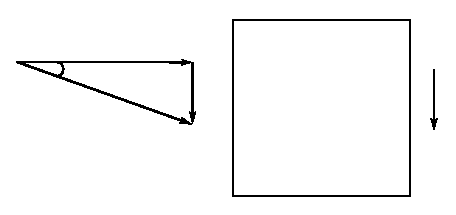
\includegraphics[width=0.5\unitlength]{./chapter-literature-revirw/fnp/setup-1.eps}}         
      
      
   
 	\put(0.315,1.04){$U$}
 	\put(0.3,0.95){$U_i$}
    \put(0.42,1.0){$\dot{y}$}
    \put(0.28,1.003){ $\theta$}
    \put(0.7,0.99){\small $(+)$}
      	

 	
 	 

     

  \end{picture}

 \caption{Induced angle of attack on a square prism due to the resultant of free-stream velocity of the fluid and transverse velocity of the body.}
    \label{fig:induced_lift_sketch}
\end{figure}

 Figure \ref{fig:induced_lift_sketch}  illustrates the motion of the body at a given instantaneous time.The induced angle of attack is formed on the square cross section as a result of the fressrteam velocity vector $U$ and the transverse velocity vector of the body $\dot{y}$. Thus, a force is formed in phase with the motion of the body (square cross section). This mechanism could also be observed on other bodies which are prone to galloping. The sign convention in this figure (and generally used in this scope of research) states that downward direction is positive. Hence, the force generated on a body under the influence of galloping, could be also identified as a ``negative lift".
 

\subsection{Qusasi-state theory}


According \cite{Paidoussis2010},the initial studies by \cite{Glauert1919} provided a criterion for galloping by considering the auto-rotation of a stalled aerofoil. As this phenomenon commonly occur in iced transmission lines, \cite{DenHartog1956} has provided a theoretical explanation for iced electric transmission lines. 

The pioneering study in order to mathematically model galloping was conducted by \cite{Parkinson1964}. This model has been widely used in almost all subsequent studies regarding galloping. A weakly non-linear oscillator model was developed by them to predict the response of the system. Essentially the quasi-steady assumption was made to develop this theory assuming that the instantaneous induced lift force of the oscillating body is equal to that of the lift force generated by the same body at the same induced angle of attack. In order to satisfy the quasi-steady assumption few conditions had to be satisfied.

\begin{itemize}
 \item The velocity of the body does not change rapidly
 \item There is no interaction between vortex shedding and galloping
\end{itemize}

The second condition is satisfied by ensuring the vortex shedding frequency is much higher than the galloping frequency.
The oscillator equation was solved using the Krylov and Bogoliubov method. Details of this method would not be mentioned as it is not used in the present study to solve the oscillator equation. The results obtained form experiments, carried out at $\reynoldsnumber=2200$ and a mass ratio (\mstar) around 1164 had a good agreement with the theoretical data which is shown in figure \ref{fig:parkinson_paper_data}.

\begin{figure}
	
  \setlength{\unitlength}{\textwidth}

        \begin{picture}(1,0.82)(0,0.4)

      % % % Parkinson Data 

      \put(0.05,0.39){\includegraphics[width=0.9\unitlength]{./chapter-literature-revirw/fnp/parkinson_data.eps}}
      
%       \put(0.07,0.95){$\displaystyle\frac{V}{D}$}
%       \put(0.07,1.3){$\displaystyle\frac{A}{D}$}
       \put(0.05,0.8){\Large$\frac{nA}{2\beta}\bar{Y}_s$}
       \put(0.52,0.42){\Large$\frac{nA}{2\beta}U$}
       \
%\put(0.189,1.415){\small(a)}
%\put(0.189,1.07){\small(b)}
%\put(0.189,0.73){\small(c)}

%  


    \end{picture}

  \caption{``Collapsed amplitude-velocity characteristic. Theory: \solidrule \ stable limit cycle, \dashedrule unstable limit cycle. Experiment $(\times) \ \beta = .00107$, $(\circ) \ \beta =.00196$,\ $(\vartriangle) \beta=.00364$,$(\triangledown) \ \beta = .00372$,\ $+1 \ \beta=.0012$,\ $+2 \ \beta=.0032$ Reynolds numbers $4,000-20,000$ ". Figure extracted from \cite{Parkinson1964}. $\frac{nA}{2\beta}\bar{Y}_s$ is the dimensionless displacement amplitude parameter and $\frac{nA}{2\beta}U$ is the reduced velocity.$\beta$ is the damping ratio and $n=\frac{1}{\mstar}$. The experimental data shows a good agreement with the theoretical model.}
    \label{fig:parkinson_paper_data}
\end{figure}

 %vspace{10cm}


\subsection{Induced force and the shear layers}

It is important to have an understanding on how the induced lift is generated in a fluid dynamics point of view. Since the quasi-steady model has already been validated and re-validated by many studies, the flow-field data of static body simulations of a square cross section, at different angle of attack is used as an example. 












  


    

     











\chapter{Methodology and validation}

\section{Introduction}
 
A brief overview of the computational methods to perform the simulations to obtain the data in this thesis are are presented in this chapter. As the this particular study is not focused on developing computational methods but concentrated on understanding the physics of a body under the influence of fluid-elastic galloping, it should be noted that the overview provided in this chapter is quite abstract.


\chapter{Influence of fluid dynamics of the system on the extracted power}

\section{Introduction}

This chapter contains the results and discussion relating to the third objective of this thesis. As discussed in chapter \ref{chap:lit-review} the induced force $F_y$ of the system is a result of the top and bottom of the shear layer behaviour of the system. The current published work shows that the afterbody of the system has a significant influence on the galloping response. In this chapter, the influence of shear layer behaviour and hence, the influence of the afterbody on mean extracted power is discussed.

Here, the influence of shear layer on the mean power is studied by introducing a cross section which is a hybrid of a square and a triangle. Data are analysed the cross section is transformed gradually by manipulating the ratio of two length scales.

The stationary forcing data is presented for each cross section followed by the QSS power curves. Based on the QSS power data, an optimum cross section for power extraction is identified. Next, the underpinning reason for the negative portion of certain $C_y$ curves is discussed through surface pressure and flow velocity data. Following this, a reasoning for the discrepancy between QSS and DNS mean power at the optimum power cross section is discussed.       

A final summary is presented explaining the influence of the shear layer on mean power output and the preliminary design considerations to optimise the fluid mechanics to obtain an optimum power output. 


\section{Influence of the shear layers}

As highlighted in section \ref{subsec:fluid_mechanics_of_galloping} the afterbody of the cross section has a significant influence on galloping. This is because of the shear layer need to interact with the afterbody after separation at the leading edge. 


The $C_y$ vs $\alpha$ curve increases reaches a maximum and reduces as the induce angle is increased. The maximum of the induced lift occurs when the separated  shear layer (at the leading edge) closer to the surface of the body reattaches at the trailing edge. Therefore, by delaying the reattachment the point where the maximum lift occurs can be shifted towards a higher induced angle which leads to a higher induced velocity. As shown in equation \ref{eqn:power_alt} higher velocity leads to higher power output. In order to test this hypothesis the shear layer reattachment was reduced by gradually tapering off the top and bottom sides of the square cross section as sown in figure \ref{fig:hybrid_section}. The $\ratio$ was changed gradually from 1 to zero at increments of 0.25 where 1 being the square cross section and 0 being an isosceles triangle.    

\begin{figure}[!h]
\setlength{\unitlength}{\textwidth}

  \begin{picture}(1,0.36)(0,0.74)
    
  \put(0.2,0.76){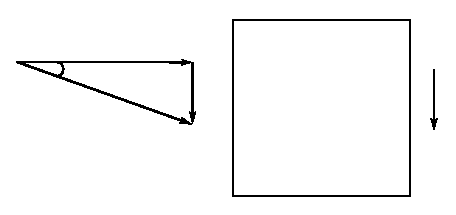
\includegraphics[width=0.5\unitlength]{./chapter-literature-revirw/fnp/setup-1.eps}}         
      
      
   
 	\put(0.315,1.04){$U$}
 	\put(0.3,0.95){$U_i$}
    \put(0.42,1.0){$\dot{y}$}
    \put(0.28,1.003){ $\theta$}
    \put(0.7,0.99){\small $(+)$}
      	

 	
 	 

     

  \end{picture}

 \caption{Induced angle of attack on a square prism due to the resultant of free-stream velocity of the fluid and transverse velocity of the body.}
    \label{fig:induced_lift_sketch}
\end{figure}

\section{Static body results}

\begin{table}[ht]

\begin{center}
\setlength{\unitlength}{\textwidth}

\begin{tabular}{c c c c c} % centered columns (4 columns)
\hline\hline %inserts double horizontal lines
\\[0.2ex]
$\ratio$ & $a_1$ & $a_3$ & $a_5$ & $a_7$ \\ [0.8ex] % inserts table 
%heading
\hline 

\\[0.8ex]% inserts single horizontal line
$0$ &  -2.30617 & -269.075 & -59.2929 & 4.74389\\[0.8ex]
    & -5.08342 & -56.5390e & -160.505e & -105.773\\[0.8ex]
    &  4.40685 & 19.9213 & 22.8894 & 7.68556\\[1ex]


\\[0.8ex]% inserts single horizontal line
$0.25$ & -0.605146 & -19.4346 &-82.4463 & -94.4226\\[0.8ex]
      & 2.50538 & 9.91021  & 10.2712 & 3.94112 \\[1ex]

 \\[0.8ex]% inserting body of the table


 $0.5$ & 1.44734 & 4.83885  & -166.900e & -983.072 \\[0.8ex]% inserting body of the table
  & 1.51455e & 15.8476 & 52.5465 & 62.8067 \\ [1ex] % [1ex] adds vertical space
  
  \\[0.8ex]% inserting body of the table
  
   $0.75$ & 1.76938 & 35.2630 & -345.562 & -10072.7 \\[0.8ex]
          & 1.77553 & 43.0120 & 262.983 & 638.484 \\ [1ex]
          
          
  
  
\hline %inserts single line


\end{tabular}

\caption{Coefficient values used in the 7th order interpolation polynomial at $Re=200$. Data present for $\ratio=0-0.75$ at increments of $0.5$. Multiples polynomials were used to attain a better fit. The plot of the compound fit is presented in figure \ref{fig:lift_curves-hybrid}.} 
 
\label{table:cy-coefficients-hybrid} % is used to refer this table in the text
\end{center}
\end{table}


\begin{figure}
  \setlength{\unitlength}{\textwidth}

  \begin{picture}(1,0.75)(0,0)
    % % %90
      % % % Parkinson Data 
      \put(0.035,0.5){\includegraphics[width=0.5\unitlength]{./chapter-cross-sections/fnp/lift_curve_sq.eps}}
      \put(0.495,0.5){\includegraphics[width=0.5\unitlength]{./chapter-cross-sections/fnp/lift_curve_075.eps}}
      \put(0.035,0.27){\includegraphics[width=0.5\unitlength]{./chapter-cross-sections/fnp/lift_curve_05.eps}}
      \put(0.495,0.27){\includegraphics[width=0.5\unitlength]{./chapter-cross-sections/fnp/lift_curve_025.eps}}
      \put(0.3,0.0){\includegraphics[width=0.5\unitlength]{./chapter-cross-sections/fnp/lift_curve_tri.eps}}
      
      
   
      
      
%      \put(0.23,0.00){ $\displaystyle\frac{c}{\rho\mathcal{A}U}$}
%      \put(0.73,0.00){ $\displaystyle\frac{c}{\rho\mathcal{A}U}$}

      \put(0.3,0.26){$\theta$}
      \put(0.76,0.26){$\theta$}
      \put(0.56,-0.01){$\theta$}
      
      \put(0.01,0.405){$\displaystyle C_y$}
       \put(0.01,0.65){$\displaystyle C_y$}
      \put(0.3,0.14){$\displaystyle C_y$}
      
      \put(0.106,0.705){\small(a)}
      \put(0.565,0.705){\small(b)}
      \put(0.106,0.475){\small(c)}
      \put(0.565,0.475){\small(d)}
      \put(0.37,0.207){\small(e)}
      

  \end{picture}

  \caption{Induced lift coefficient $C_y$ at different angles for selected cross sections. Data presented for cross sections, (a) square, (b) $\ratio=0.75$, (c) $\ratio=0.5$, (d) $\ratio=0.25$ and (e) triangle.}
  \label{fig:lift_curves-hybrid}
\end{figure}

% !TeX spellcheck = en_GB
\begin{figure}[!htb]
  \setlength{\unitlength}{\textwidth}

        \begin{picture}(1,0.4)(-0.02,0)

 
      
      \put(0.08,0.02){\includegraphics[width=0.75\unitlength]{./FnP/mean_power_hyb.eps}}

      \put(0.46,0.00){\massdamp}
      
      
     
       \put(0.03,0.235){$\displaystyle\frac{P_{m}}{\rho \mathcal{A}U^3 }$}
      

      %\put(0.095,0.218){\small(a)}
      %\put(0.565,0.218){\small(b)}
      
    \end{picture}

  \caption{Dimensionless mean power obtained using QSS model as a function of \massdamp. Data presented for five selected cross sections, square ($\triangle$), $\ratio=0.75$ (+), $\ratio=0.5$ (\ding{117}), $\ratio=0.25$ ($\times$) and triangle (\ding{108}) at $\reynoldsnumber=200$, $\massstiff=100$.}
    \label{fig:power_curves}
\end{figure}

 %vspace{10cm}

\begin{figure}
  \setlength{\unitlength}{\textwidth}

        \begin{picture}(1,1.1)(0,0.35)

      % % % Parkinson Data 
      \put(0.1,1.1){\includegraphics[width=0.75\unitlength]{./chapter-cross-sections/fnp/surf-pres-tri-4.eps}}
      \put(0.1,0.737){\includegraphics[width=0.75\unitlength]{./chapter-cross-sections/fnp/surf-pres-tri-16.eps}}
      \put(0.1,0.38){\includegraphics[width=0.75\unitlength]{./chapter-cross-sections/fnp/surf-pres-tri-21.eps}}
     
      
      



%      
    \put(0.21,1.41){\small(a)}
     \put(0.21,1.05){\small(b)}
     \put(0.21,0.69){\small(c)}
\put(0.1,0.95){$\displaystyle P_{s}$}
\put(0.1,1.3){$\displaystyle P_{s}$}
\put(0.1,0.56){$\displaystyle P_{s}$}
\put(0.26,0.35){Relative destance from the leading edge}

      
    \end{picture}

    \caption{Surface pressure of top (\ding{83}) and bottom (\ding{117})  surfaces of the static triangular cross section at (a) $\theta=4^\circ$, (b) $\theta=16^\circ$ \ and (c) $\theta=21^\circ$ A clear pressure difference is visible between the surfaces. The top surface comparatively has more negative pressure where a lift is created which results in a negative $C_y$ at $4^\circ$ and reduces as $\theta$ \ is increased, while the vice versa occurs at the top surface.}
    \label{fig:surf_pres}
\end{figure}

 %vspace{10cm}

\begin{figure}[!htb]
\setlength{\unitlength}{\textwidth}

  \begin{picture}(1,0.38)(0,0.74)
    
  \put(0.32,0.76){\includegraphics[width=0.32\unitlength]{./chapter-cross-sections/fnp/tri-sketch.eps}}         
      
      
   
 %	\put(0.28,0.937){$\theta$}
 	%\put(0.52,0.74){$l$}
   

 	
 	 

     

  \end{picture}

 \caption{Illustration of the lines along which the flow velocity magnitudes have been extracted. The data have been extracted along a line starting from the separation points in the outward direction (shown with arrows) for the top and bottom surfaces.}
    \label{fig:tri-sketch}
\end{figure}
\begin{figure}[!h]
  \setlength{\unitlength}{\textwidth}

        \begin{picture}(1,1.1)(0,0.35)

      % % % Parkinson Data 
      \put(0.1,1.1){\includegraphics[width=0.75\unitlength]{./chapter-cross-sections/fnp/vel_prof-tri-4.eps}}
      \put(0.1,0.737){\includegraphics[width=0.75\unitlength]{./chapter-cross-sections/fnp/vel_prof-tri-16.eps}}
      \put(0.1,0.38){\includegraphics[width=0.75\unitlength]{./chapter-cross-sections/fnp/vel_prof-tri-21.eps}}
     
      
      



%      
    \put(0.21,1.41){\small(a)}
     \put(0.21,1.05){\small(b)}
     \put(0.21,0.69){\small(c)}
\put(0.1,0.95){$\displaystyle V_m$}
\put(0.1,1.3){$\displaystyle V_m$}
\put(0.1,0.56){$\displaystyle V_m$}
\put(0.34,0.35){Distance from the leading edge}

      
    \end{picture}

    \caption{Velocity magnitudes of the flow along a line parallel to the front surface spreading towards top (\dashedrule) and bottom (\solidrule) boundaries (figure \ref{fig:tri-sketch}). These two lines (for the top and bottom surfaces) start from the top and bottom leading edges of the triangular cross section. Data present (a) $\alpha=4^\circ$, (b) $\alpha=16^\circ$ \ and (c) $\alpha=21^\circ$.}
    \label{fig:vel-profile}
\end{figure}

 %vspace{10cm}

% !TeX spellcheck = en_GB
\begin{figure}[!htb]
  \setlength{\unitlength}{\textwidth}

        \begin{picture}(1,0.4)(-0.02,0)

 
      
      \put(0.08,0.02){\includegraphics[width=0.75\unitlength]{./chapter-cross-sections/fnp/fsi_flow_sketch.eps}}

      %\put(0.46,0.00){\massdamp}
      
      
     
       %\put(0.03,0.235){$\displaystyle\frac{P_{m}}{\rho \mathcal{A}U^3 }$}
      

      %\put(0.095,0.218){\small(a)}
      %\put(0.565,0.218){\small(b)}
      
    \end{picture}

  \caption{}
    \label{fig:power_curves}
\end{figure}

 %vspace{10cm}

\begin{figure}[!htb]
  \setlength{\unitlength}{\textwidth}

  \begin{picture}(1,1.2)(0,0)
    % % %90
      % % % Parkinson Data 
      \put(0.005,0.8){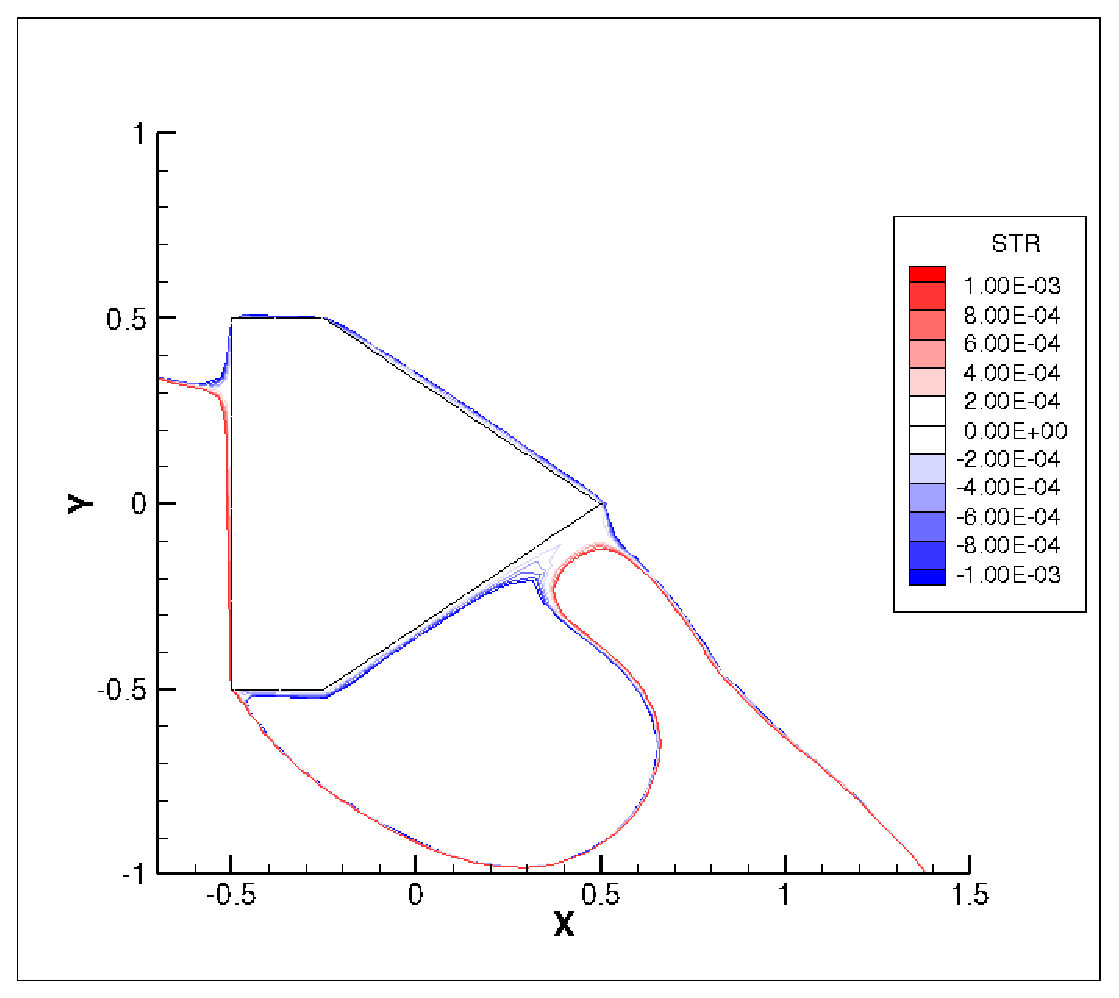
\includegraphics[width=0.4\unitlength]{./chapter-cross-sections/fnp/fsi-0.25-1.eps}}
      \put(0.005,0.4){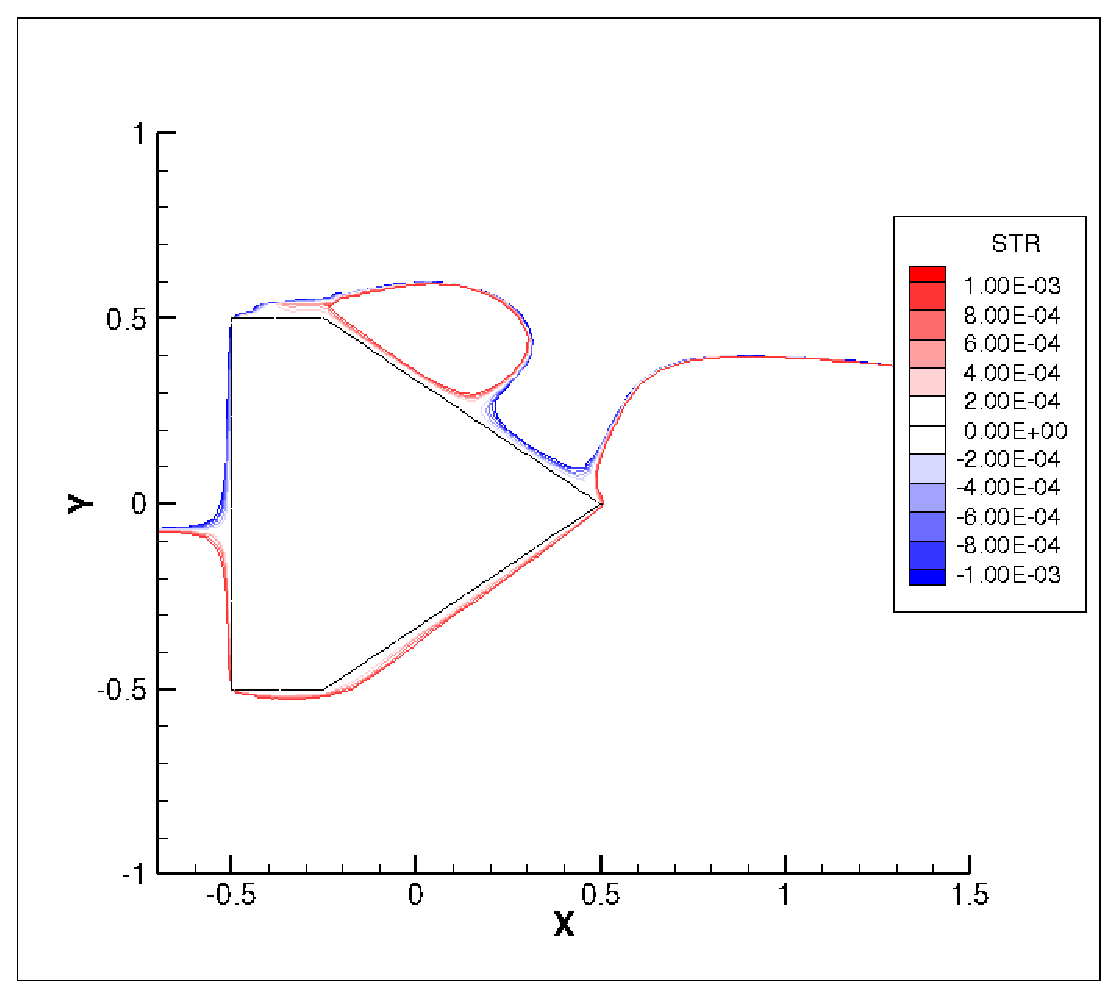
\includegraphics[width=0.4\unitlength]{./chapter-cross-sections/fnp/fsi-0.25-2.eps}}
      \put(0.005,0.0){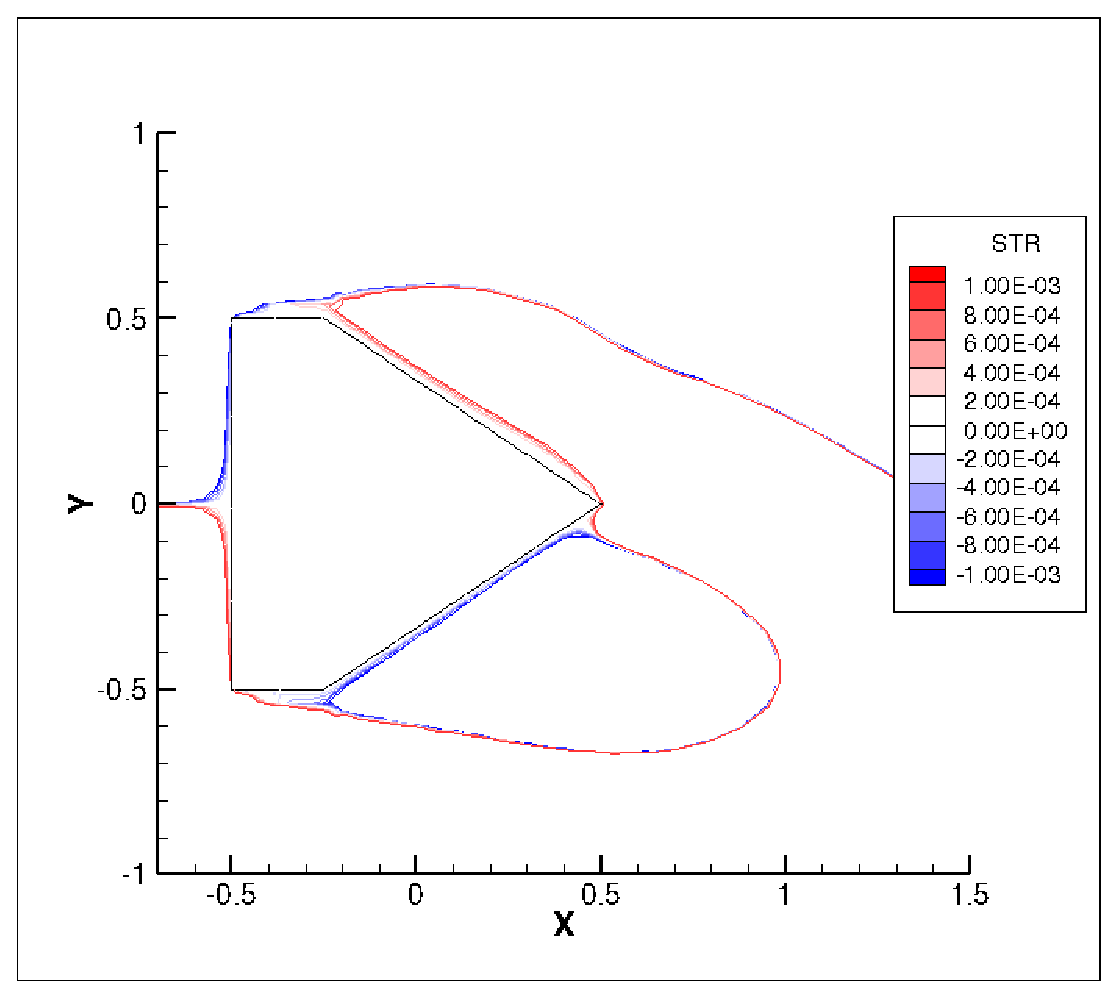
\includegraphics[width=0.4\unitlength]{./chapter-cross-sections/fnp/fsi-0.25-3.eps}}

      
      
      \put(0.505,0.8){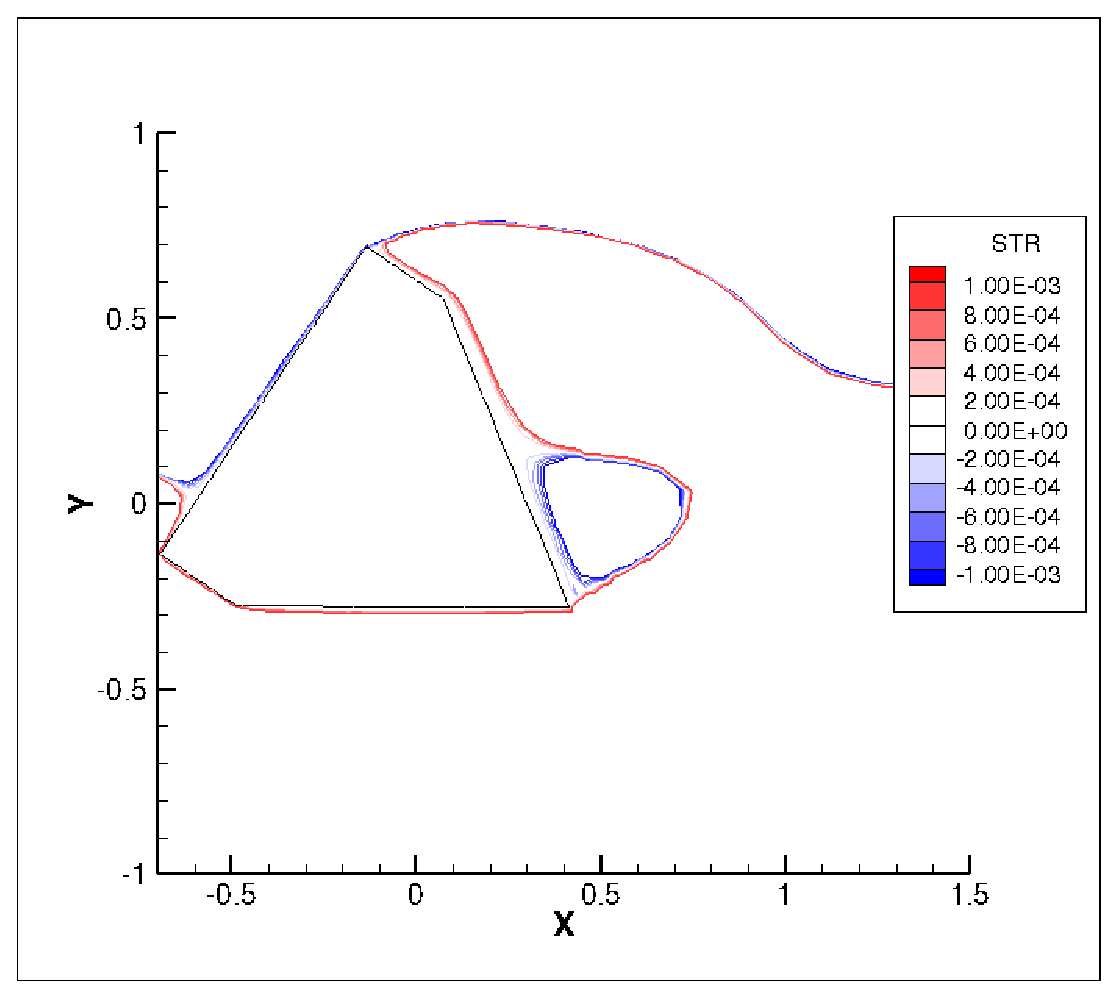
\includegraphics[width=0.4\unitlength]{./chapter-cross-sections/fnp/qss-0.25-1.eps}}
      \put(0.505,0.4){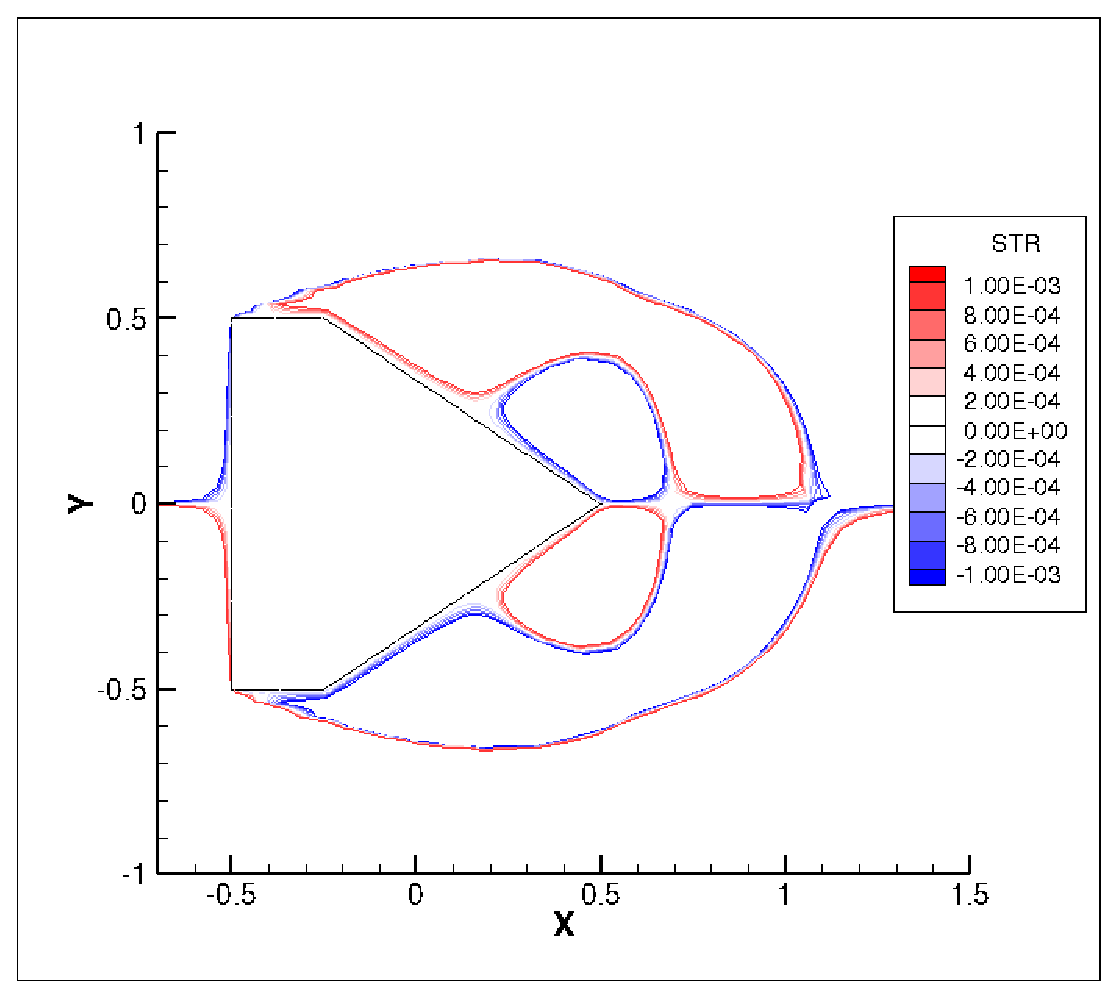
\includegraphics[width=0.4\unitlength]{./chapter-cross-sections/fnp/qss-0.25-3.eps}}
      \put(0.505,0.0){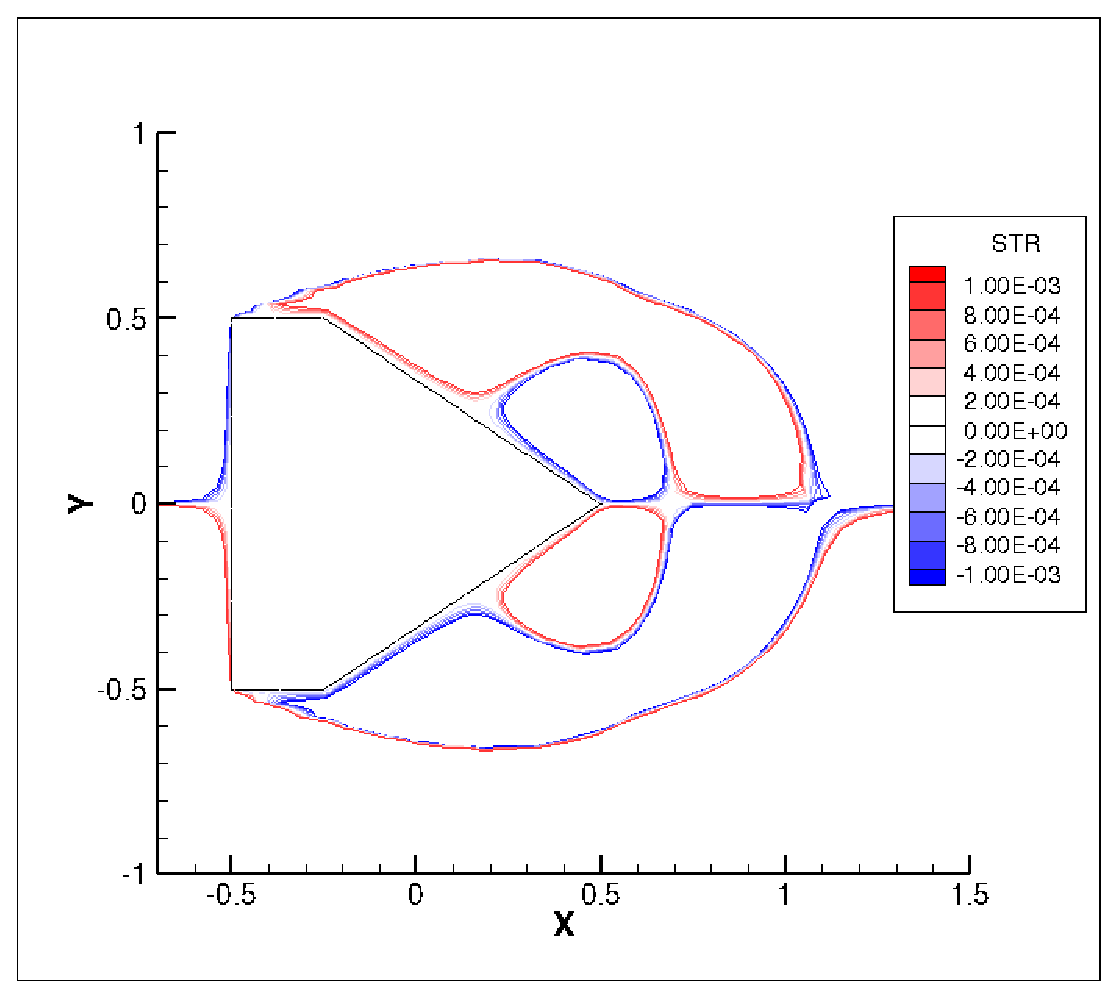
\includegraphics[width=0.4\unitlength]{./chapter-cross-sections/fnp/qss-0.25-3.eps}} 
      
      
%      \put(0.23,0.00){ $\displaystyle\frac{c}{\rho\mathcal{A}U}$}
%      \put(0.73,0.00){ $\displaystyle\frac{c}{\rho\mathcal{A}U}$}


      
      \put(0.01,1.125){\small(a)}
      \put(0.510,1.125){\small(b)}
      \put(0.01,0.725){\small(c)}
      \put(0.510,0.725){\small(d)}
      \put(0.01,0.33){\small(e)}
      \put(0.510,0.33){\small(f)}
      
   
   
      

  \end{picture}

  \caption{Time averaged stream functions of stationary and oscillating flow-fields of the hybrid cross section ($\ratio=0.25$), averaged over a vortex shedding cycle. (a), (c) and (e) the averaged stream functions of the oscillating case at $t=2295.763$ (point 1), $t=2305.897$ (point 2) and $t=2325.870$ (point 3) . (b), (d) and (f) are the stream functions of the flow field of the stationary body corresponding to the induced angles of (a), (c) and (e).}  
  \label{fig:flow_field_FSI}
\end{figure}


\chapter{Influence of fluid dynamics of the system on the extracted power}

\section{Introduction}

This chapter contains the results and discussion relating to the third objective of this thesis. As discussed in chapter \ref{chap:lit-review} the induced force $F_y$ of the system is a result of the top and bottom of the shear layer behaviour of the system. The current published work shows that the afterbody of the system has a significant influence on the galloping response. In this chapter, the influence of shear layer behaviour and hence, the influence of the afterbody on mean extracted power is discussed.

Here, the influence of shear layer on the mean power is studied by introducing a cross section which is a hybrid of a square and a triangle. Data are analysed the cross section is transformed gradually by manipulating the ratio of two length scales.

The stationary forcing data is presented for each cross section followed by the QSS power curves. Based on the QSS power data, an optimum cross section for power extraction is identified. Next, the underpinning reason for the negative portion of certain $C_y$ curves is discussed through surface pressure and flow velocity data. Following this, a reasoning for the discrepancy between QSS and DNS mean power at the optimum power cross section is discussed.       

A final summary is presented explaining the influence of the shear layer on mean power output and the preliminary design considerations to optimise the fluid mechanics to obtain an optimum power output. 


\section{Influence of the shear layers}

As highlighted in section \ref{subsec:fluid_mechanics_of_galloping} the afterbody of the cross section has a significant influence on galloping. This is because of the shear layer need to interact with the afterbody after separation at the leading edge. 


The $C_y$ vs $\alpha$ curve increases reaches a maximum and reduces as the induce angle is increased. The maximum of the induced lift occurs when the separated  shear layer (at the leading edge) closer to the surface of the body reattaches at the trailing edge. Therefore, by delaying the reattachment the point where the maximum lift occurs can be shifted towards a higher induced angle which leads to a higher induced velocity. As shown in equation \ref{eqn:power_alt} higher velocity leads to higher power output. In order to test this hypothesis the shear layer reattachment was reduced by gradually tapering off the top and bottom sides of the square cross section as sown in figure \ref{fig:hybrid_section}. The $\ratio$ was changed gradually from 1 to zero at increments of 0.25 where 1 being the square cross section and 0 being an isosceles triangle.    

\begin{figure}[!h]
\setlength{\unitlength}{\textwidth}

  \begin{picture}(1,0.36)(0,0.74)
    
  \put(0.2,0.76){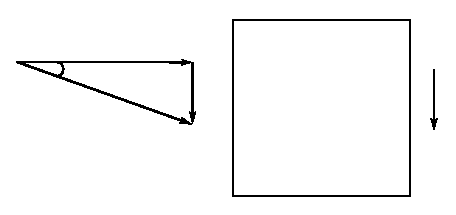
\includegraphics[width=0.5\unitlength]{./chapter-literature-revirw/fnp/setup-1.eps}}         
      
      
   
 	\put(0.315,1.04){$U$}
 	\put(0.3,0.95){$U_i$}
    \put(0.42,1.0){$\dot{y}$}
    \put(0.28,1.003){ $\theta$}
    \put(0.7,0.99){\small $(+)$}
      	

 	
 	 

     

  \end{picture}

 \caption{Induced angle of attack on a square prism due to the resultant of free-stream velocity of the fluid and transverse velocity of the body.}
    \label{fig:induced_lift_sketch}
\end{figure}

\section{Static body results}

\begin{table}[ht]

\begin{center}
\setlength{\unitlength}{\textwidth}

\begin{tabular}{c c c c c} % centered columns (4 columns)
\hline\hline %inserts double horizontal lines
\\[0.2ex]
$\ratio$ & $a_1$ & $a_3$ & $a_5$ & $a_7$ \\ [0.8ex] % inserts table 
%heading
\hline 

\\[0.8ex]% inserts single horizontal line
$0$ &  -2.30617 & -269.075 & -59.2929 & 4.74389\\[0.8ex]
    & -5.08342 & -56.5390e & -160.505e & -105.773\\[0.8ex]
    &  4.40685 & 19.9213 & 22.8894 & 7.68556\\[1ex]


\\[0.8ex]% inserts single horizontal line
$0.25$ & -0.605146 & -19.4346 &-82.4463 & -94.4226\\[0.8ex]
      & 2.50538 & 9.91021  & 10.2712 & 3.94112 \\[1ex]

 \\[0.8ex]% inserting body of the table


 $0.5$ & 1.44734 & 4.83885  & -166.900e & -983.072 \\[0.8ex]% inserting body of the table
  & 1.51455e & 15.8476 & 52.5465 & 62.8067 \\ [1ex] % [1ex] adds vertical space
  
  \\[0.8ex]% inserting body of the table
  
   $0.75$ & 1.76938 & 35.2630 & -345.562 & -10072.7 \\[0.8ex]
          & 1.77553 & 43.0120 & 262.983 & 638.484 \\ [1ex]
          
          
  
  
\hline %inserts single line


\end{tabular}

\caption{Coefficient values used in the 7th order interpolation polynomial at $Re=200$. Data present for $\ratio=0-0.75$ at increments of $0.5$. Multiples polynomials were used to attain a better fit. The plot of the compound fit is presented in figure \ref{fig:lift_curves-hybrid}.} 
 
\label{table:cy-coefficients-hybrid} % is used to refer this table in the text
\end{center}
\end{table}


\begin{figure}
  \setlength{\unitlength}{\textwidth}

  \begin{picture}(1,0.75)(0,0)
    % % %90
      % % % Parkinson Data 
      \put(0.035,0.5){\includegraphics[width=0.5\unitlength]{./chapter-cross-sections/fnp/lift_curve_sq.eps}}
      \put(0.495,0.5){\includegraphics[width=0.5\unitlength]{./chapter-cross-sections/fnp/lift_curve_075.eps}}
      \put(0.035,0.27){\includegraphics[width=0.5\unitlength]{./chapter-cross-sections/fnp/lift_curve_05.eps}}
      \put(0.495,0.27){\includegraphics[width=0.5\unitlength]{./chapter-cross-sections/fnp/lift_curve_025.eps}}
      \put(0.3,0.0){\includegraphics[width=0.5\unitlength]{./chapter-cross-sections/fnp/lift_curve_tri.eps}}
      
      
   
      
      
%      \put(0.23,0.00){ $\displaystyle\frac{c}{\rho\mathcal{A}U}$}
%      \put(0.73,0.00){ $\displaystyle\frac{c}{\rho\mathcal{A}U}$}

      \put(0.3,0.26){$\theta$}
      \put(0.76,0.26){$\theta$}
      \put(0.56,-0.01){$\theta$}
      
      \put(0.01,0.405){$\displaystyle C_y$}
       \put(0.01,0.65){$\displaystyle C_y$}
      \put(0.3,0.14){$\displaystyle C_y$}
      
      \put(0.106,0.705){\small(a)}
      \put(0.565,0.705){\small(b)}
      \put(0.106,0.475){\small(c)}
      \put(0.565,0.475){\small(d)}
      \put(0.37,0.207){\small(e)}
      

  \end{picture}

  \caption{Induced lift coefficient $C_y$ at different angles for selected cross sections. Data presented for cross sections, (a) square, (b) $\ratio=0.75$, (c) $\ratio=0.5$, (d) $\ratio=0.25$ and (e) triangle.}
  \label{fig:lift_curves-hybrid}
\end{figure}

% !TeX spellcheck = en_GB
\begin{figure}[!htb]
  \setlength{\unitlength}{\textwidth}

        \begin{picture}(1,0.4)(-0.02,0)

 
      
      \put(0.08,0.02){\includegraphics[width=0.75\unitlength]{./FnP/mean_power_hyb.eps}}

      \put(0.46,0.00){\massdamp}
      
      
     
       \put(0.03,0.235){$\displaystyle\frac{P_{m}}{\rho \mathcal{A}U^3 }$}
      

      %\put(0.095,0.218){\small(a)}
      %\put(0.565,0.218){\small(b)}
      
    \end{picture}

  \caption{Dimensionless mean power obtained using QSS model as a function of \massdamp. Data presented for five selected cross sections, square ($\triangle$), $\ratio=0.75$ (+), $\ratio=0.5$ (\ding{117}), $\ratio=0.25$ ($\times$) and triangle (\ding{108}) at $\reynoldsnumber=200$, $\massstiff=100$.}
    \label{fig:power_curves}
\end{figure}

 %vspace{10cm}

\begin{figure}
  \setlength{\unitlength}{\textwidth}

        \begin{picture}(1,1.1)(0,0.35)

      % % % Parkinson Data 
      \put(0.1,1.1){\includegraphics[width=0.75\unitlength]{./chapter-cross-sections/fnp/surf-pres-tri-4.eps}}
      \put(0.1,0.737){\includegraphics[width=0.75\unitlength]{./chapter-cross-sections/fnp/surf-pres-tri-16.eps}}
      \put(0.1,0.38){\includegraphics[width=0.75\unitlength]{./chapter-cross-sections/fnp/surf-pres-tri-21.eps}}
     
      
      



%      
    \put(0.21,1.41){\small(a)}
     \put(0.21,1.05){\small(b)}
     \put(0.21,0.69){\small(c)}
\put(0.1,0.95){$\displaystyle P_{s}$}
\put(0.1,1.3){$\displaystyle P_{s}$}
\put(0.1,0.56){$\displaystyle P_{s}$}
\put(0.26,0.35){Relative destance from the leading edge}

      
    \end{picture}

    \caption{Surface pressure of top (\ding{83}) and bottom (\ding{117})  surfaces of the static triangular cross section at (a) $\theta=4^\circ$, (b) $\theta=16^\circ$ \ and (c) $\theta=21^\circ$ A clear pressure difference is visible between the surfaces. The top surface comparatively has more negative pressure where a lift is created which results in a negative $C_y$ at $4^\circ$ and reduces as $\theta$ \ is increased, while the vice versa occurs at the top surface.}
    \label{fig:surf_pres}
\end{figure}

 %vspace{10cm}

\begin{figure}[!htb]
\setlength{\unitlength}{\textwidth}

  \begin{picture}(1,0.38)(0,0.74)
    
  \put(0.32,0.76){\includegraphics[width=0.32\unitlength]{./chapter-cross-sections/fnp/tri-sketch.eps}}         
      
      
   
 %	\put(0.28,0.937){$\theta$}
 	%\put(0.52,0.74){$l$}
   

 	
 	 

     

  \end{picture}

 \caption{Illustration of the lines along which the flow velocity magnitudes have been extracted. The data have been extracted along a line starting from the separation points in the outward direction (shown with arrows) for the top and bottom surfaces.}
    \label{fig:tri-sketch}
\end{figure}
\begin{figure}[!h]
  \setlength{\unitlength}{\textwidth}

        \begin{picture}(1,1.1)(0,0.35)

      % % % Parkinson Data 
      \put(0.1,1.1){\includegraphics[width=0.75\unitlength]{./chapter-cross-sections/fnp/vel_prof-tri-4.eps}}
      \put(0.1,0.737){\includegraphics[width=0.75\unitlength]{./chapter-cross-sections/fnp/vel_prof-tri-16.eps}}
      \put(0.1,0.38){\includegraphics[width=0.75\unitlength]{./chapter-cross-sections/fnp/vel_prof-tri-21.eps}}
     
      
      



%      
    \put(0.21,1.41){\small(a)}
     \put(0.21,1.05){\small(b)}
     \put(0.21,0.69){\small(c)}
\put(0.1,0.95){$\displaystyle V_m$}
\put(0.1,1.3){$\displaystyle V_m$}
\put(0.1,0.56){$\displaystyle V_m$}
\put(0.34,0.35){Distance from the leading edge}

      
    \end{picture}

    \caption{Velocity magnitudes of the flow along a line parallel to the front surface spreading towards top (\dashedrule) and bottom (\solidrule) boundaries (figure \ref{fig:tri-sketch}). These two lines (for the top and bottom surfaces) start from the top and bottom leading edges of the triangular cross section. Data present (a) $\alpha=4^\circ$, (b) $\alpha=16^\circ$ \ and (c) $\alpha=21^\circ$.}
    \label{fig:vel-profile}
\end{figure}

 %vspace{10cm}

% !TeX spellcheck = en_GB
\begin{figure}[!htb]
  \setlength{\unitlength}{\textwidth}

        \begin{picture}(1,0.4)(-0.02,0)

 
      
      \put(0.08,0.02){\includegraphics[width=0.75\unitlength]{./chapter-cross-sections/fnp/fsi_flow_sketch.eps}}

      %\put(0.46,0.00){\massdamp}
      
      
     
       %\put(0.03,0.235){$\displaystyle\frac{P_{m}}{\rho \mathcal{A}U^3 }$}
      

      %\put(0.095,0.218){\small(a)}
      %\put(0.565,0.218){\small(b)}
      
    \end{picture}

  \caption{}
    \label{fig:power_curves}
\end{figure}

 %vspace{10cm}

\begin{figure}[!htb]
  \setlength{\unitlength}{\textwidth}

  \begin{picture}(1,1.2)(0,0)
    % % %90
      % % % Parkinson Data 
      \put(0.005,0.8){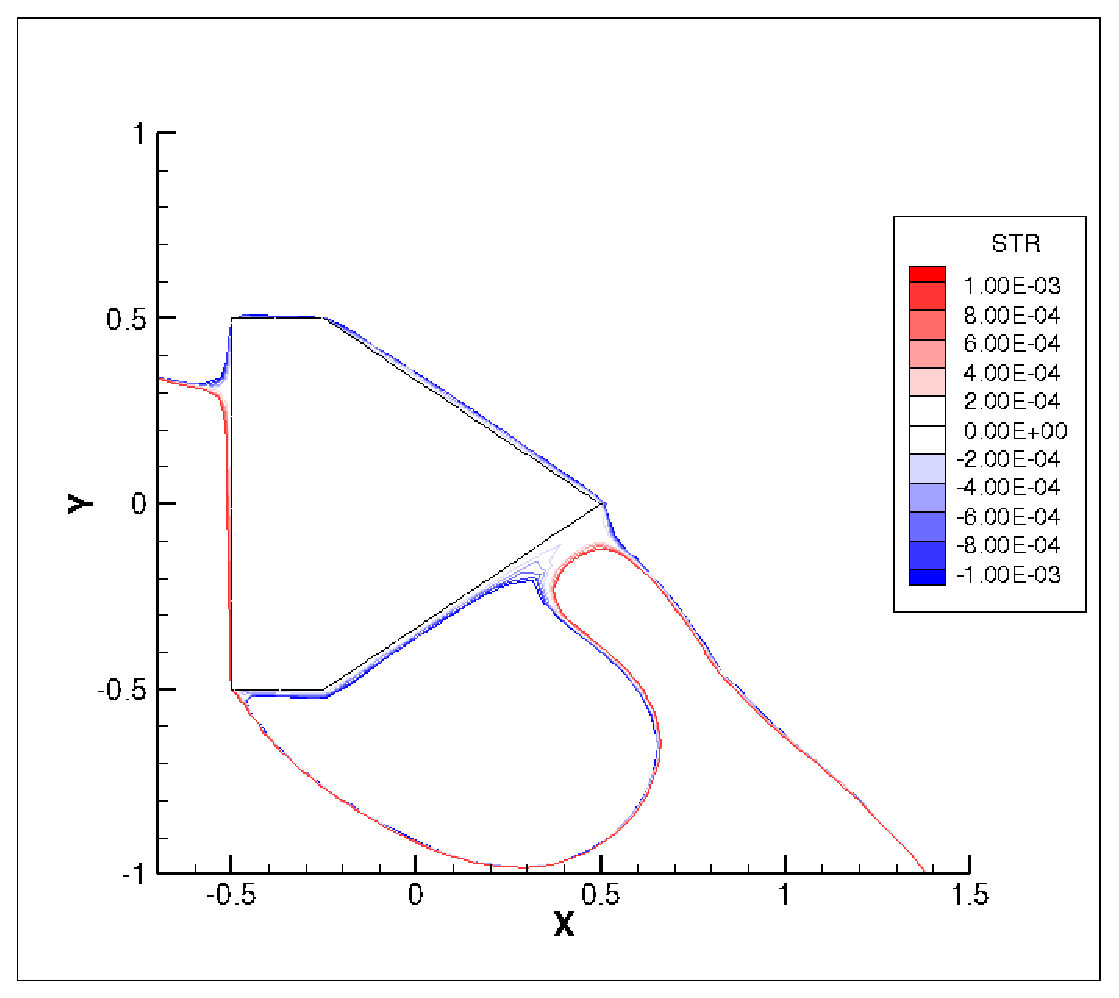
\includegraphics[width=0.4\unitlength]{./chapter-cross-sections/fnp/fsi-0.25-1.eps}}
      \put(0.005,0.4){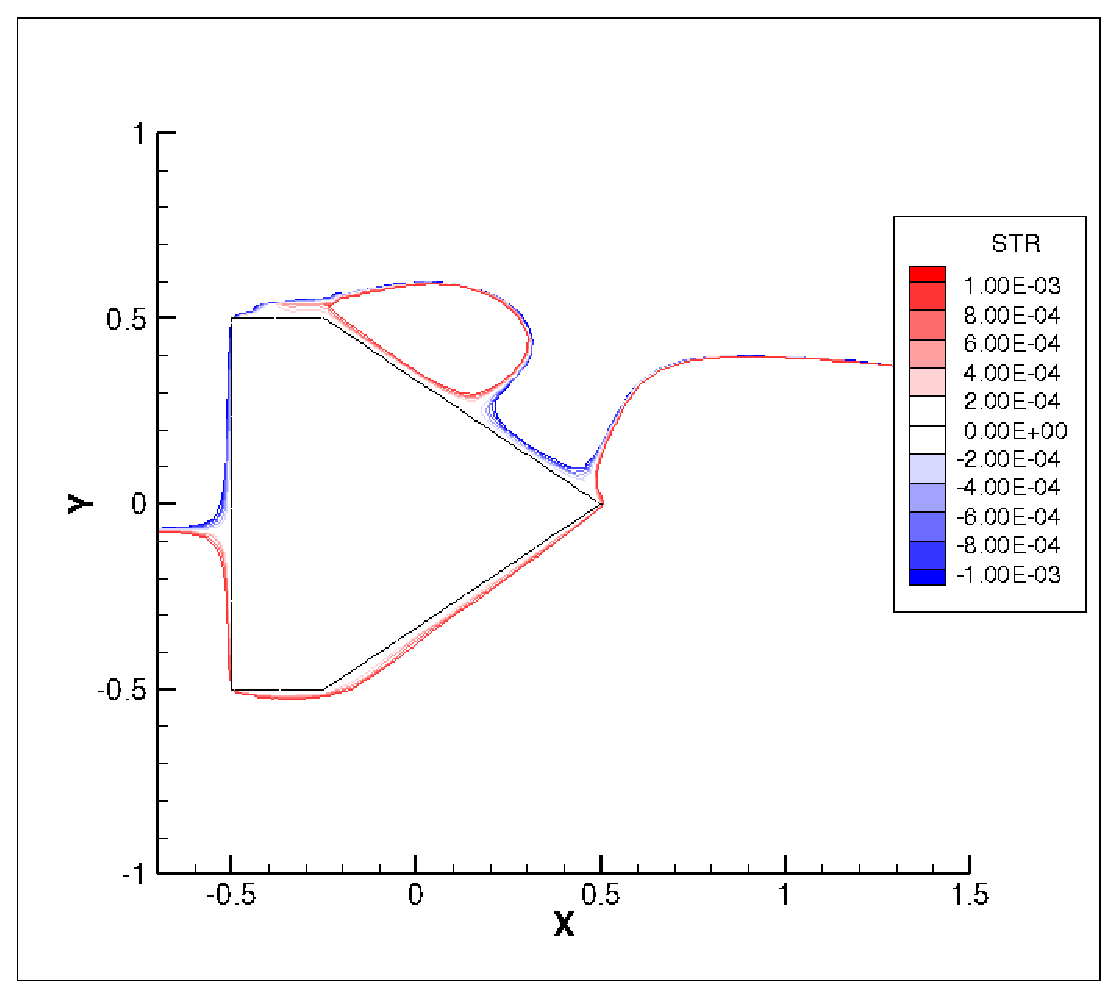
\includegraphics[width=0.4\unitlength]{./chapter-cross-sections/fnp/fsi-0.25-2.eps}}
      \put(0.005,0.0){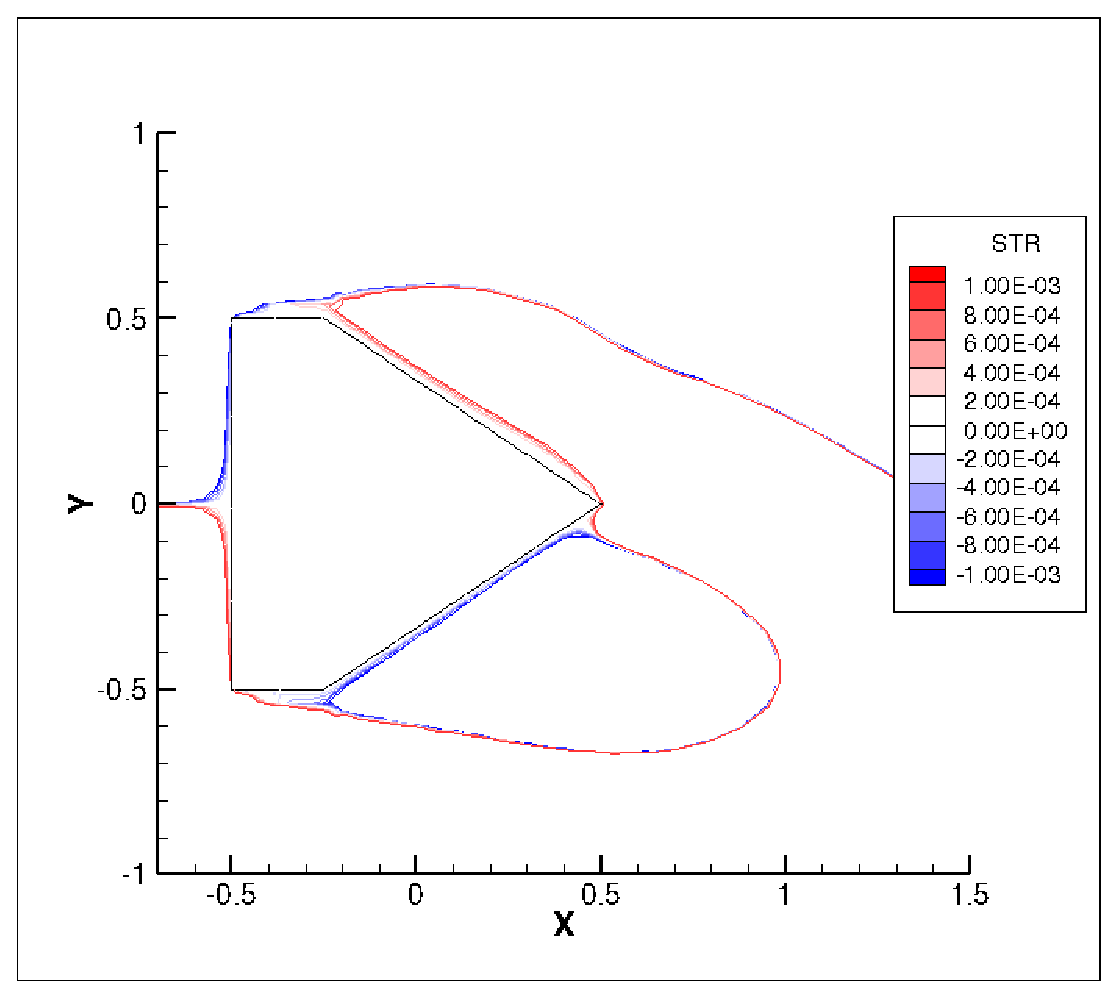
\includegraphics[width=0.4\unitlength]{./chapter-cross-sections/fnp/fsi-0.25-3.eps}}

      
      
      \put(0.505,0.8){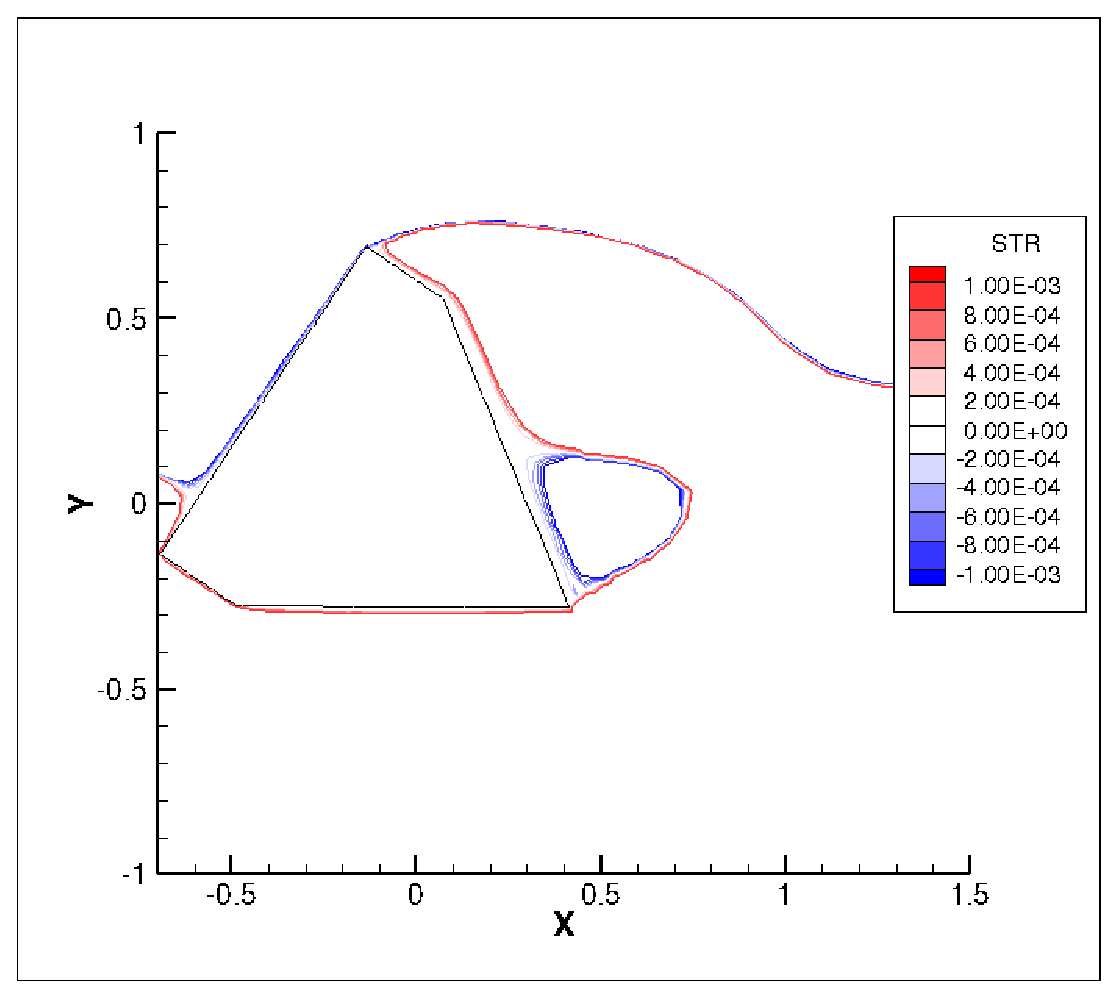
\includegraphics[width=0.4\unitlength]{./chapter-cross-sections/fnp/qss-0.25-1.eps}}
      \put(0.505,0.4){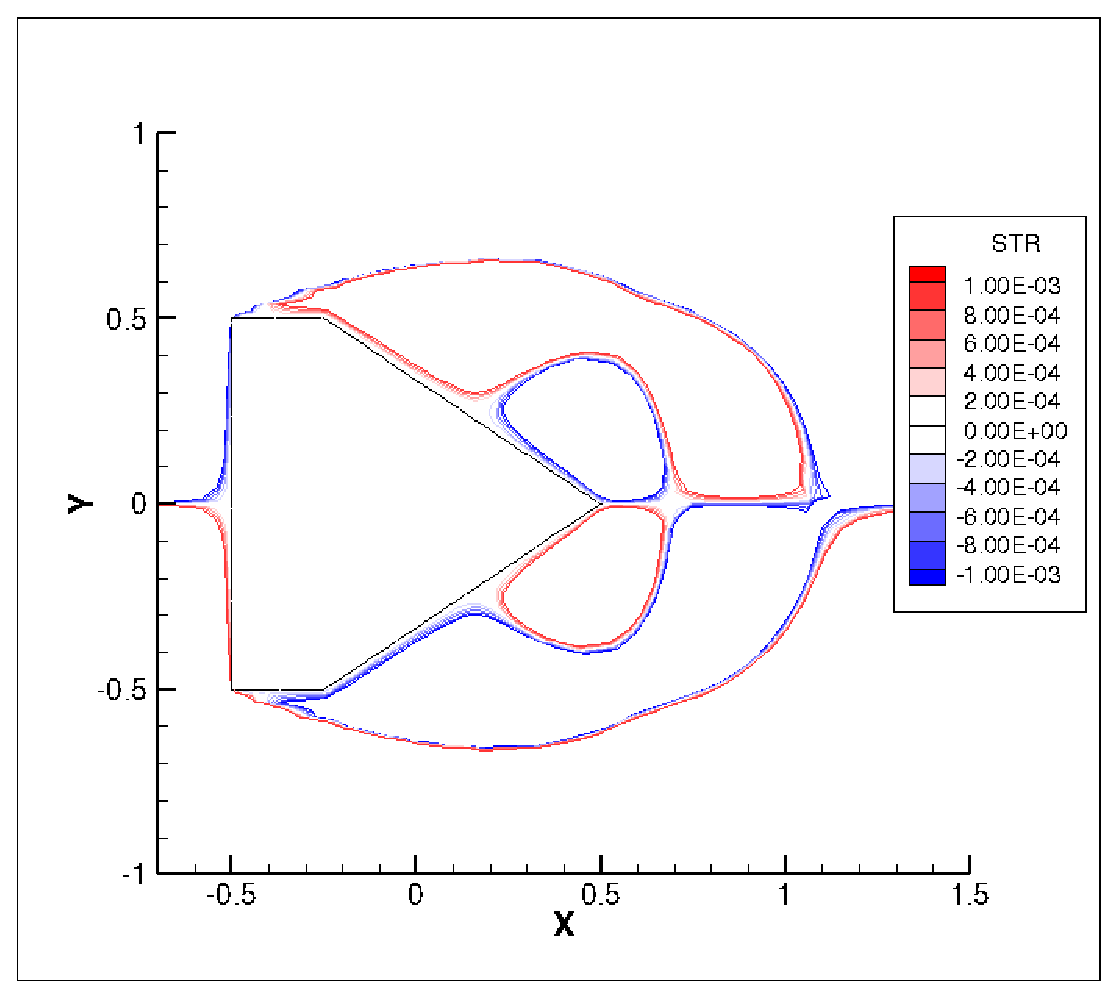
\includegraphics[width=0.4\unitlength]{./chapter-cross-sections/fnp/qss-0.25-3.eps}}
      \put(0.505,0.0){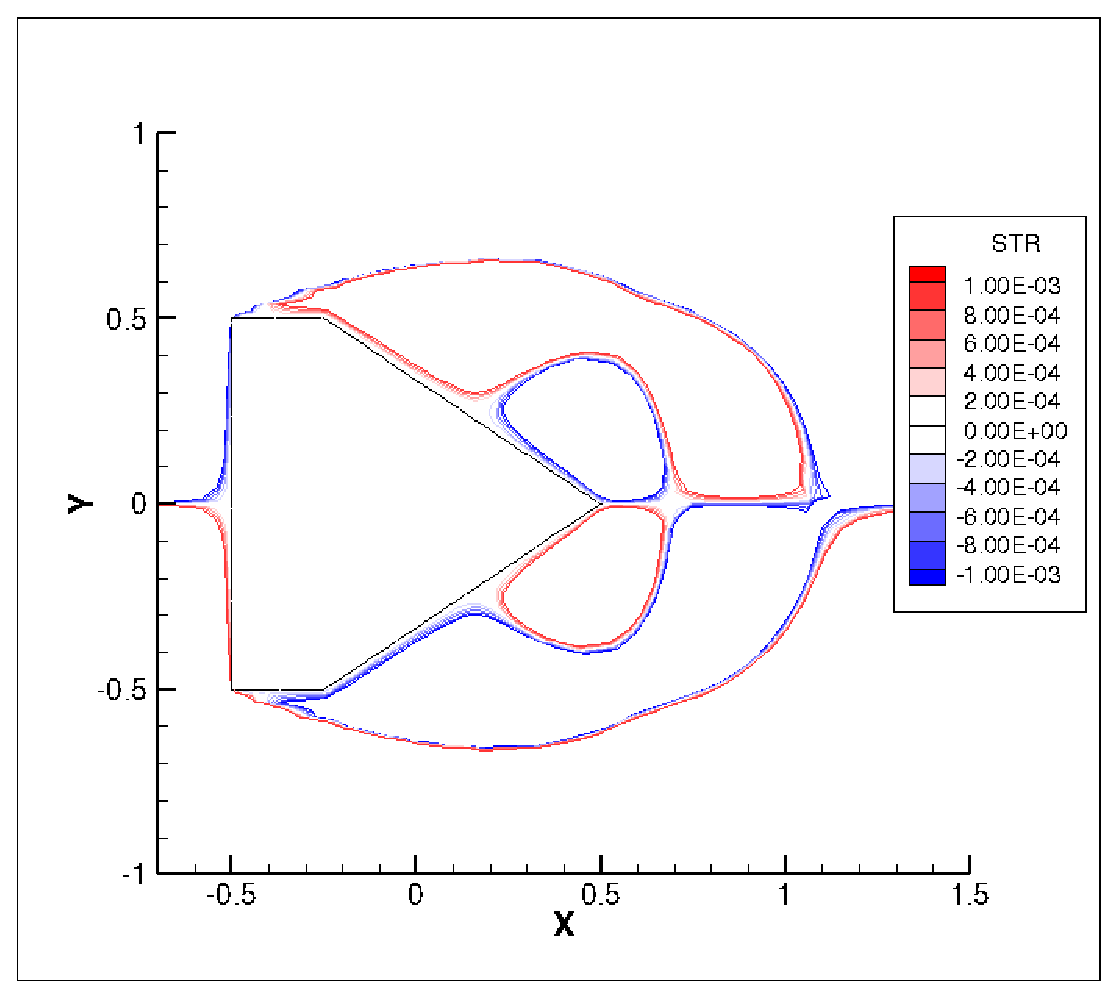
\includegraphics[width=0.4\unitlength]{./chapter-cross-sections/fnp/qss-0.25-3.eps}} 
      
      
%      \put(0.23,0.00){ $\displaystyle\frac{c}{\rho\mathcal{A}U}$}
%      \put(0.73,0.00){ $\displaystyle\frac{c}{\rho\mathcal{A}U}$}


      
      \put(0.01,1.125){\small(a)}
      \put(0.510,1.125){\small(b)}
      \put(0.01,0.725){\small(c)}
      \put(0.510,0.725){\small(d)}
      \put(0.01,0.33){\small(e)}
      \put(0.510,0.33){\small(f)}
      
   
   
      

  \end{picture}

  \caption{Time averaged stream functions of stationary and oscillating flow-fields of the hybrid cross section ($\ratio=0.25$), averaged over a vortex shedding cycle. (a), (c) and (e) the averaged stream functions of the oscillating case at $t=2295.763$ (point 1), $t=2305.897$ (point 2) and $t=2325.870$ (point 3) . (b), (d) and (f) are the stream functions of the flow field of the stationary body corresponding to the induced angles of (a), (c) and (e).}  
  \label{fig:flow_field_FSI}
\end{figure}


\chapter{Influence of fluid dynamics of the system on the extracted power}

\section{Introduction}

This chapter contains the results and discussion relating to the third objective of this thesis. As discussed in chapter \ref{chap:lit-review} the induced force $F_y$ of the system is a result of the top and bottom of the shear layer behaviour of the system. The current published work shows that the afterbody of the system has a significant influence on the galloping response. In this chapter, the influence of shear layer behaviour and hence, the influence of the afterbody on mean extracted power is discussed.

Here, the influence of shear layer on the mean power is studied by introducing a cross section which is a hybrid of a square and a triangle. Data are analysed the cross section is transformed gradually by manipulating the ratio of two length scales.

The stationary forcing data is presented for each cross section followed by the QSS power curves. Based on the QSS power data, an optimum cross section for power extraction is identified. Next, the underpinning reason for the negative portion of certain $C_y$ curves is discussed through surface pressure and flow velocity data. Following this, a reasoning for the discrepancy between QSS and DNS mean power at the optimum power cross section is discussed.       

A final summary is presented explaining the influence of the shear layer on mean power output and the preliminary design considerations to optimise the fluid mechanics to obtain an optimum power output. 


\section{Influence of the shear layers}

As highlighted in section \ref{subsec:fluid_mechanics_of_galloping} the afterbody of the cross section has a significant influence on galloping. This is because of the shear layer need to interact with the afterbody after separation at the leading edge. 


The $C_y$ vs $\alpha$ curve increases reaches a maximum and reduces as the induce angle is increased. The maximum of the induced lift occurs when the separated  shear layer (at the leading edge) closer to the surface of the body reattaches at the trailing edge. Therefore, by delaying the reattachment the point where the maximum lift occurs can be shifted towards a higher induced angle which leads to a higher induced velocity. As shown in equation \ref{eqn:power_alt} higher velocity leads to higher power output. In order to test this hypothesis the shear layer reattachment was reduced by gradually tapering off the top and bottom sides of the square cross section as sown in figure \ref{fig:hybrid_section}. The $\ratio$ was changed gradually from 1 to zero at increments of 0.25 where 1 being the square cross section and 0 being an isosceles triangle.    

\begin{figure}[!h]
\setlength{\unitlength}{\textwidth}

  \begin{picture}(1,0.36)(0,0.74)
    
  \put(0.2,0.76){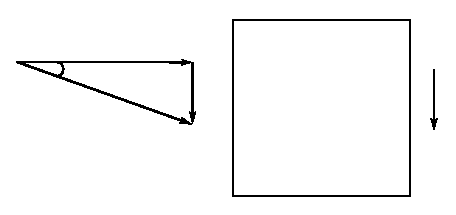
\includegraphics[width=0.5\unitlength]{./chapter-literature-revirw/fnp/setup-1.eps}}         
      
      
   
 	\put(0.315,1.04){$U$}
 	\put(0.3,0.95){$U_i$}
    \put(0.42,1.0){$\dot{y}$}
    \put(0.28,1.003){ $\theta$}
    \put(0.7,0.99){\small $(+)$}
      	

 	
 	 

     

  \end{picture}

 \caption{Induced angle of attack on a square prism due to the resultant of free-stream velocity of the fluid and transverse velocity of the body.}
    \label{fig:induced_lift_sketch}
\end{figure}

\section{Static body results}

\begin{table}[ht]

\begin{center}
\setlength{\unitlength}{\textwidth}

\begin{tabular}{c c c c c} % centered columns (4 columns)
\hline\hline %inserts double horizontal lines
\\[0.2ex]
$\ratio$ & $a_1$ & $a_3$ & $a_5$ & $a_7$ \\ [0.8ex] % inserts table 
%heading
\hline 

\\[0.8ex]% inserts single horizontal line
$0$ &  -2.30617 & -269.075 & -59.2929 & 4.74389\\[0.8ex]
    & -5.08342 & -56.5390e & -160.505e & -105.773\\[0.8ex]
    &  4.40685 & 19.9213 & 22.8894 & 7.68556\\[1ex]


\\[0.8ex]% inserts single horizontal line
$0.25$ & -0.605146 & -19.4346 &-82.4463 & -94.4226\\[0.8ex]
      & 2.50538 & 9.91021  & 10.2712 & 3.94112 \\[1ex]

 \\[0.8ex]% inserting body of the table


 $0.5$ & 1.44734 & 4.83885  & -166.900e & -983.072 \\[0.8ex]% inserting body of the table
  & 1.51455e & 15.8476 & 52.5465 & 62.8067 \\ [1ex] % [1ex] adds vertical space
  
  \\[0.8ex]% inserting body of the table
  
   $0.75$ & 1.76938 & 35.2630 & -345.562 & -10072.7 \\[0.8ex]
          & 1.77553 & 43.0120 & 262.983 & 638.484 \\ [1ex]
          
          
  
  
\hline %inserts single line


\end{tabular}

\caption{Coefficient values used in the 7th order interpolation polynomial at $Re=200$. Data present for $\ratio=0-0.75$ at increments of $0.5$. Multiples polynomials were used to attain a better fit. The plot of the compound fit is presented in figure \ref{fig:lift_curves-hybrid}.} 
 
\label{table:cy-coefficients-hybrid} % is used to refer this table in the text
\end{center}
\end{table}


\begin{figure}
  \setlength{\unitlength}{\textwidth}

  \begin{picture}(1,0.75)(0,0)
    % % %90
      % % % Parkinson Data 
      \put(0.035,0.5){\includegraphics[width=0.5\unitlength]{./chapter-cross-sections/fnp/lift_curve_sq.eps}}
      \put(0.495,0.5){\includegraphics[width=0.5\unitlength]{./chapter-cross-sections/fnp/lift_curve_075.eps}}
      \put(0.035,0.27){\includegraphics[width=0.5\unitlength]{./chapter-cross-sections/fnp/lift_curve_05.eps}}
      \put(0.495,0.27){\includegraphics[width=0.5\unitlength]{./chapter-cross-sections/fnp/lift_curve_025.eps}}
      \put(0.3,0.0){\includegraphics[width=0.5\unitlength]{./chapter-cross-sections/fnp/lift_curve_tri.eps}}
      
      
   
      
      
%      \put(0.23,0.00){ $\displaystyle\frac{c}{\rho\mathcal{A}U}$}
%      \put(0.73,0.00){ $\displaystyle\frac{c}{\rho\mathcal{A}U}$}

      \put(0.3,0.26){$\theta$}
      \put(0.76,0.26){$\theta$}
      \put(0.56,-0.01){$\theta$}
      
      \put(0.01,0.405){$\displaystyle C_y$}
       \put(0.01,0.65){$\displaystyle C_y$}
      \put(0.3,0.14){$\displaystyle C_y$}
      
      \put(0.106,0.705){\small(a)}
      \put(0.565,0.705){\small(b)}
      \put(0.106,0.475){\small(c)}
      \put(0.565,0.475){\small(d)}
      \put(0.37,0.207){\small(e)}
      

  \end{picture}

  \caption{Induced lift coefficient $C_y$ at different angles for selected cross sections. Data presented for cross sections, (a) square, (b) $\ratio=0.75$, (c) $\ratio=0.5$, (d) $\ratio=0.25$ and (e) triangle.}
  \label{fig:lift_curves-hybrid}
\end{figure}

% !TeX spellcheck = en_GB
\begin{figure}[!htb]
  \setlength{\unitlength}{\textwidth}

        \begin{picture}(1,0.4)(-0.02,0)

 
      
      \put(0.08,0.02){\includegraphics[width=0.75\unitlength]{./FnP/mean_power_hyb.eps}}

      \put(0.46,0.00){\massdamp}
      
      
     
       \put(0.03,0.235){$\displaystyle\frac{P_{m}}{\rho \mathcal{A}U^3 }$}
      

      %\put(0.095,0.218){\small(a)}
      %\put(0.565,0.218){\small(b)}
      
    \end{picture}

  \caption{Dimensionless mean power obtained using QSS model as a function of \massdamp. Data presented for five selected cross sections, square ($\triangle$), $\ratio=0.75$ (+), $\ratio=0.5$ (\ding{117}), $\ratio=0.25$ ($\times$) and triangle (\ding{108}) at $\reynoldsnumber=200$, $\massstiff=100$.}
    \label{fig:power_curves}
\end{figure}

 %vspace{10cm}

\begin{figure}
  \setlength{\unitlength}{\textwidth}

        \begin{picture}(1,1.1)(0,0.35)

      % % % Parkinson Data 
      \put(0.1,1.1){\includegraphics[width=0.75\unitlength]{./chapter-cross-sections/fnp/surf-pres-tri-4.eps}}
      \put(0.1,0.737){\includegraphics[width=0.75\unitlength]{./chapter-cross-sections/fnp/surf-pres-tri-16.eps}}
      \put(0.1,0.38){\includegraphics[width=0.75\unitlength]{./chapter-cross-sections/fnp/surf-pres-tri-21.eps}}
     
      
      



%      
    \put(0.21,1.41){\small(a)}
     \put(0.21,1.05){\small(b)}
     \put(0.21,0.69){\small(c)}
\put(0.1,0.95){$\displaystyle P_{s}$}
\put(0.1,1.3){$\displaystyle P_{s}$}
\put(0.1,0.56){$\displaystyle P_{s}$}
\put(0.26,0.35){Relative destance from the leading edge}

      
    \end{picture}

    \caption{Surface pressure of top (\ding{83}) and bottom (\ding{117})  surfaces of the static triangular cross section at (a) $\theta=4^\circ$, (b) $\theta=16^\circ$ \ and (c) $\theta=21^\circ$ A clear pressure difference is visible between the surfaces. The top surface comparatively has more negative pressure where a lift is created which results in a negative $C_y$ at $4^\circ$ and reduces as $\theta$ \ is increased, while the vice versa occurs at the top surface.}
    \label{fig:surf_pres}
\end{figure}

 %vspace{10cm}

\begin{figure}[!htb]
\setlength{\unitlength}{\textwidth}

  \begin{picture}(1,0.38)(0,0.74)
    
  \put(0.32,0.76){\includegraphics[width=0.32\unitlength]{./chapter-cross-sections/fnp/tri-sketch.eps}}         
      
      
   
 %	\put(0.28,0.937){$\theta$}
 	%\put(0.52,0.74){$l$}
   

 	
 	 

     

  \end{picture}

 \caption{Illustration of the lines along which the flow velocity magnitudes have been extracted. The data have been extracted along a line starting from the separation points in the outward direction (shown with arrows) for the top and bottom surfaces.}
    \label{fig:tri-sketch}
\end{figure}
\begin{figure}[!h]
  \setlength{\unitlength}{\textwidth}

        \begin{picture}(1,1.1)(0,0.35)

      % % % Parkinson Data 
      \put(0.1,1.1){\includegraphics[width=0.75\unitlength]{./chapter-cross-sections/fnp/vel_prof-tri-4.eps}}
      \put(0.1,0.737){\includegraphics[width=0.75\unitlength]{./chapter-cross-sections/fnp/vel_prof-tri-16.eps}}
      \put(0.1,0.38){\includegraphics[width=0.75\unitlength]{./chapter-cross-sections/fnp/vel_prof-tri-21.eps}}
     
      
      



%      
    \put(0.21,1.41){\small(a)}
     \put(0.21,1.05){\small(b)}
     \put(0.21,0.69){\small(c)}
\put(0.1,0.95){$\displaystyle V_m$}
\put(0.1,1.3){$\displaystyle V_m$}
\put(0.1,0.56){$\displaystyle V_m$}
\put(0.34,0.35){Distance from the leading edge}

      
    \end{picture}

    \caption{Velocity magnitudes of the flow along a line parallel to the front surface spreading towards top (\dashedrule) and bottom (\solidrule) boundaries (figure \ref{fig:tri-sketch}). These two lines (for the top and bottom surfaces) start from the top and bottom leading edges of the triangular cross section. Data present (a) $\alpha=4^\circ$, (b) $\alpha=16^\circ$ \ and (c) $\alpha=21^\circ$.}
    \label{fig:vel-profile}
\end{figure}

 %vspace{10cm}

% !TeX spellcheck = en_GB
\begin{figure}[!htb]
  \setlength{\unitlength}{\textwidth}

        \begin{picture}(1,0.4)(-0.02,0)

 
      
      \put(0.08,0.02){\includegraphics[width=0.75\unitlength]{./chapter-cross-sections/fnp/fsi_flow_sketch.eps}}

      %\put(0.46,0.00){\massdamp}
      
      
     
       %\put(0.03,0.235){$\displaystyle\frac{P_{m}}{\rho \mathcal{A}U^3 }$}
      

      %\put(0.095,0.218){\small(a)}
      %\put(0.565,0.218){\small(b)}
      
    \end{picture}

  \caption{}
    \label{fig:power_curves}
\end{figure}

 %vspace{10cm}

\begin{figure}[!htb]
  \setlength{\unitlength}{\textwidth}

  \begin{picture}(1,1.2)(0,0)
    % % %90
      % % % Parkinson Data 
      \put(0.005,0.8){\includegraphics[width=0.4\unitlength]{./chapter-cross-sections/fnp/fsi-0.25-1.eps}}
      \put(0.005,0.4){\includegraphics[width=0.4\unitlength]{./chapter-cross-sections/fnp/fsi-0.25-2.eps}}
      \put(0.005,0.0){\includegraphics[width=0.4\unitlength]{./chapter-cross-sections/fnp/fsi-0.25-3.eps}}

      
      
      \put(0.505,0.8){\includegraphics[width=0.4\unitlength]{./chapter-cross-sections/fnp/qss-0.25-1.eps}}
      \put(0.505,0.4){\includegraphics[width=0.4\unitlength]{./chapter-cross-sections/fnp/qss-0.25-3.eps}}
      \put(0.505,0.0){\includegraphics[width=0.4\unitlength]{./chapter-cross-sections/fnp/qss-0.25-3.eps}} 
      
      
%      \put(0.23,0.00){ $\displaystyle\frac{c}{\rho\mathcal{A}U}$}
%      \put(0.73,0.00){ $\displaystyle\frac{c}{\rho\mathcal{A}U}$}


      
      \put(0.01,1.125){\small(a)}
      \put(0.510,1.125){\small(b)}
      \put(0.01,0.725){\small(c)}
      \put(0.510,0.725){\small(d)}
      \put(0.01,0.33){\small(e)}
      \put(0.510,0.33){\small(f)}
      
   
   
      

  \end{picture}

  \caption{Time averaged stream functions of stationary and oscillating flow-fields of the hybrid cross section ($\ratio=0.25$), averaged over a vortex shedding cycle. (a), (c) and (e) the averaged stream functions of the oscillating case at $t=2295.763$ (point 1), $t=2305.897$ (point 2) and $t=2325.870$ (point 3) . (b), (d) and (f) are the stream functions of the flow field of the stationary body corresponding to the induced angles of (a), (c) and (e).}  
  \label{fig:flow_field_FSI}
\end{figure}


\chapter{Conclusions}

A fundamental study was carried out to explore the potential of obtaining useful energy from fluid-elastic galloping. This research was based on numerical models and simulations. The study was primarily focused on understanding the energy transfer between the fluid and the structure.  

As previously mentioned, since  galloping was a fluid-structure mechanism two major objectives were identified for research namely, Understanding the underpinning structural parameters of the system and methods to optimise it for a better power output and understanding the fluid mechanics of the system and thereby obtain an optimum mean power output by controlling these mechanics. A third sub-objective was identified during the study of the first objective, which was to carry out a brief study of the frequency response to compliment the first objective of this research.  

New governing dimensionless groups for galloping namely, \massstiff\ and \massdamp\ were formulated using the natural times-scales of the linearised quasi-steady state model. Data were obtained using a square cross section. The formulated dimensionless groups provided a good collapse for the predicted power output in comparison with the classical VIV parameters which have been traditionally used i.e. \ustar\ and $\zeta$. The collapsed dimensionless groups reinforces the argument the velocity amplitude to the system and the power transfer of the system does not depend on the natural frequency of the system over a large range of natural frequencies. Although equation \ref{eqn:eom_nondim_regroup_pi_1_pi_2} shows that \mstar\ is an independent parameter, the data show that the system is essentially a function of \massstiff\ and \massdamp. A close inspection of equation \ref{eqn:eom_nondim_regroup_pi_1_pi_2} reveals that \mstar\ only has an impact on the non-linear forcing terms in relation to the velocity of the body. Thus in order for these non-linear terms to be acceptable, the the induced angle of attack and therefore, the velocity of the body needs to be very large, which appears not to be the case for the rage of parameters which were tested. 

 It could be concluded through comparison between the quasi-steady state and direct numerical simulation data, that the quasi-steady state model provides a good approximation of the power output of the system when \massstiff\ is relatively high. However, the QSS approximation is to close at low values of \massstiff\ due to the fact that QSS model does not account for the impact of vortex shedding which is shown to increase in influence as \massstiff\ is decreased. Be that as it may, the QSS model does provide a reasonable prediction of the value of \massdamp\ at which maximum power is produced. Both the error in predicted maximum power between the QSS and the DNS models and the relative power of the vortex shedding have been quantified and scale similar to $1/\sqrt{\massstiff}$  
 
 A brief frequency study was carried out in order to complement the understanding of \massstiff\ and \massdamp. Using the eigenvalues of the system an expression for galloping frequency was formulated in terms of \massstiff\ and \massdamp. This frequency was defined as the linear frequency \freqlin\ of the system. Based on this frequency two regions of frequency response was identified which were the linear frequency rage where $f_{lin}$>0 and the non-linear range where $f_{lin}=0$. Both frequency data obtained using QSS model and DNS agreed well with \freqlin\ within the boundaries of the DNS simulations where lower boundary of \massstiff\ was limited to $\massstiff=10$ due to the weakening of the galloping signal.
 
 The QSS frequency data tend to deviate from the linear frequency beyond $\massstiff<10$. Implying the start of the influence of the non-linear forcing. 
 
 The QSS model kept providing a signal and hence a frequency in the non-linear frequency region. Thus, the comparison parameter was the unstamped natural frequency as \freqlin$=0$ and \freqdns could not be obtained from the signal processing techniques used. The data showed and acceptable agreement between $0.06\geq$ but deviated as \massstiff\ reduced.
 
 The mere existence of this non-linear frequency region was a question as no DNS data could be obtained, because the galloping signal was weak and the techniques used to obtain the  frequency was not sensitive enough to capture these weak signals. Thus it was concluded that further investigations should be carried out on this region but was not pursed in this study due to deviation of the major objective and scope and time constrains.
 
 Yet, The linear expression of the galloping frequency formulated using \massstiff\ and \massdamp\ provided a excellent prediction within the boundaries where DNS data were obtained. This complimented the overall understanding and of the new formulated parameters \massstiff\ and \massdamp, completing the first objective of and the first phase of this research, \emph{``Understanding the governing mechanical parameters of the system and isolate regions where a good power transfer could be obtained."}
 
 The second phase or the objective of this study was focused on optimisation of the governing fluid mechanics of the system in order to obtain a higher power output. The primary hypothesis was that delaying the flow re-attachment would lead to a higher power output. The square cross section was systematically tapered off by changing the \ratio\ ratio in order to achieve this.
 
 One interesting observation was the presence of a negative region of the \cy vs. $\theta$ curve beyond $\ratio\leq0$. Thus, a loss of power could be observed in a certain portion of the galloping cycle was present as due to the fact that the velocity and the transverse forcing $F_{y}$ was out of phase. 
 
 It was observed that the maximum mean power increases as \ratio\ was degreased until $\ratio=0.25$. However, further analysis revealed that the maximum power at $\ratio=0.25$ was grater than $\ratio=0$ which was a direct result of the size of the negative region of the \cy\ vs. $\theta$ curve. Thus it could be concluded that the initial hypothesis could be proven but with some conditions.  
 
 Further investigation of the surface pressure data and the velocity magnitude data revealed that the changes in flow velocities at the separation points, as a result of the shape of the cross section and the incidence angle caused this negative region of the \cy plot. 
 
 Comparison of QSS maximum power data and FSI data provided similar trends of maximum power being increased as $\ratio$ was increased proving the initial hypothesis. However, the error between the QSS and FSI maximum power data increased exponentially as \ratio\ reduced. Investigations carried out using time averaged flow-filed data concluded that the mean flow of the FSI simulations had a significant deviation with the corresponding stationary DNS data. This was a result of the incurred higher  traverse velocities as \ratio\ was decreased. AS a result significant non-linear forcing was present resulting a deviation from the quasi-steady hypothesis. Be that as it may, as concluded is phase one of this study QSS model could be used as a tool to obtain initial qualitative approximations to design galloping energy harvesting systems. 
 
 It could be concluded that a key design consideration in obtaining a obtain an optimum cross section for energy harvesting is to find a good balance between the negative and positive regions of the \cy\ vs. $\theta$ curve. Delaying reattachment is beneficial however, the presence of the negative region of the \cy\ curve will have a adverse effect on power transfer. 
 
 Future research and development was also discussed in this phase. A further design considerations could be considered, for example, investigating the possibility of reducing the negative region of the \cy curve by making alterations to the cross section such as rounding the edges of flow separation.
 
 Therefore, the second phase was concluded and the second objective of this study was achieved which was:\emph{ ``Understand the governing fluid mechanics of the system and to optimise and control these mechanics in order to obtain a higher power transfer."}
 
 
 
 

\myclearpage

\bibliographystyle{elsarticle-harv}
\bibliography{./Paper.bib}
\end{document}

